\documentclass[10pt]{beamer}

\setbeamertemplate{note page}[default]
%\setbeameroption{hide notes}
\setbeameroption{show notes}


\usetheme[progressbar=frametitle]{metropolis}
\usepackage{appendixnumberbeamer}

\usepackage{booktabs}
\usepackage[scale=2]{ccicons}

\usepackage{pgfplots}
\usepgfplotslibrary{dateplot}
\usepackage{multicol}
\setlength{\columnsep}{1.5cm}

\usepackage{animate}
\usepackage{lmodern}
\usepackage[T1]{fontenc}
\usepackage{mathtools}
\usepackage{graphicx}
\usepackage{caption}
\usepackage[export]{adjustbox}

\definecolor{set1}{RGB}{228, 26, 28}
\definecolor{set2}{RGB}{77, 175, 74}
\definecolor{set3}{RGB}{255, 127, 0}
\definecolor{set4}{RGB}{166, 86, 40}
\definecolor{set5}{RGB}{153, 153, 153}

\usepackage{xspace}
\newcommand{\themename}{\textbf{\textsc{metropolis}}\xspace}

\newcommand\Fontvi{\fontsize{8}{9}\selectfont}
\newcommand\Fontvr{\fontsize{6}{7}\selectfont}

\setbeamerfont{parent A}{size=\small}


\title{Introduction to Machine Learning}
\subtitle{Digital Transformation of Healthcare}
% \date{\today}
\date{}
\author{Michoel Snow M.D. Ph.D. and Glen Ferguson Ph.D.}
\institute{Center for Health Data Innovations}
% \titlegraphic{\hfill\includegraphics[height=1.5cm]{logo.pdf}}

\begin{document}

\maketitle

\section{Intro to Machine Learning}

\begin{frame}{Bioinformatics Pipeline}
	\begin{center}
		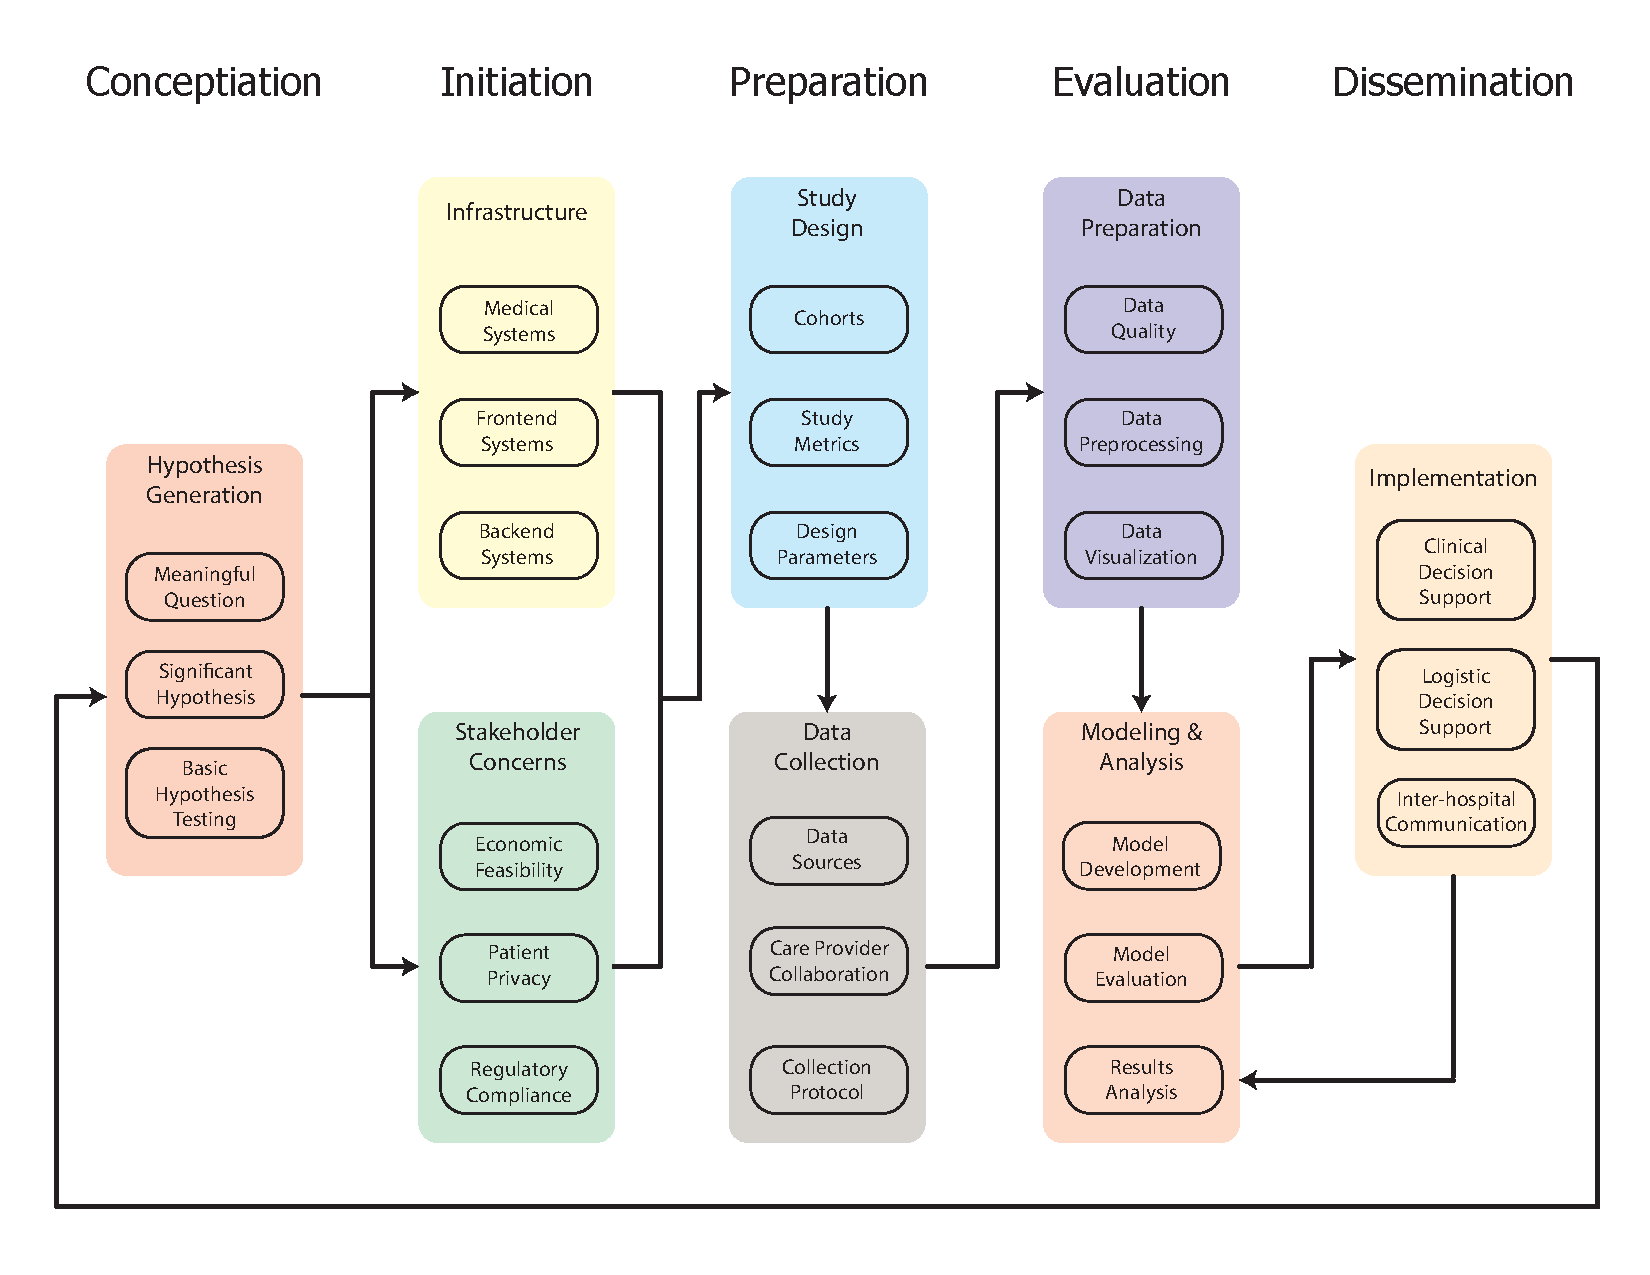
\includegraphics[width=0.8\textwidth]{images/informatics_pipeline.pdf}	
	\end{center}
\end{frame}


\begin{frame}{Data Analysis}
	\begin{center}
		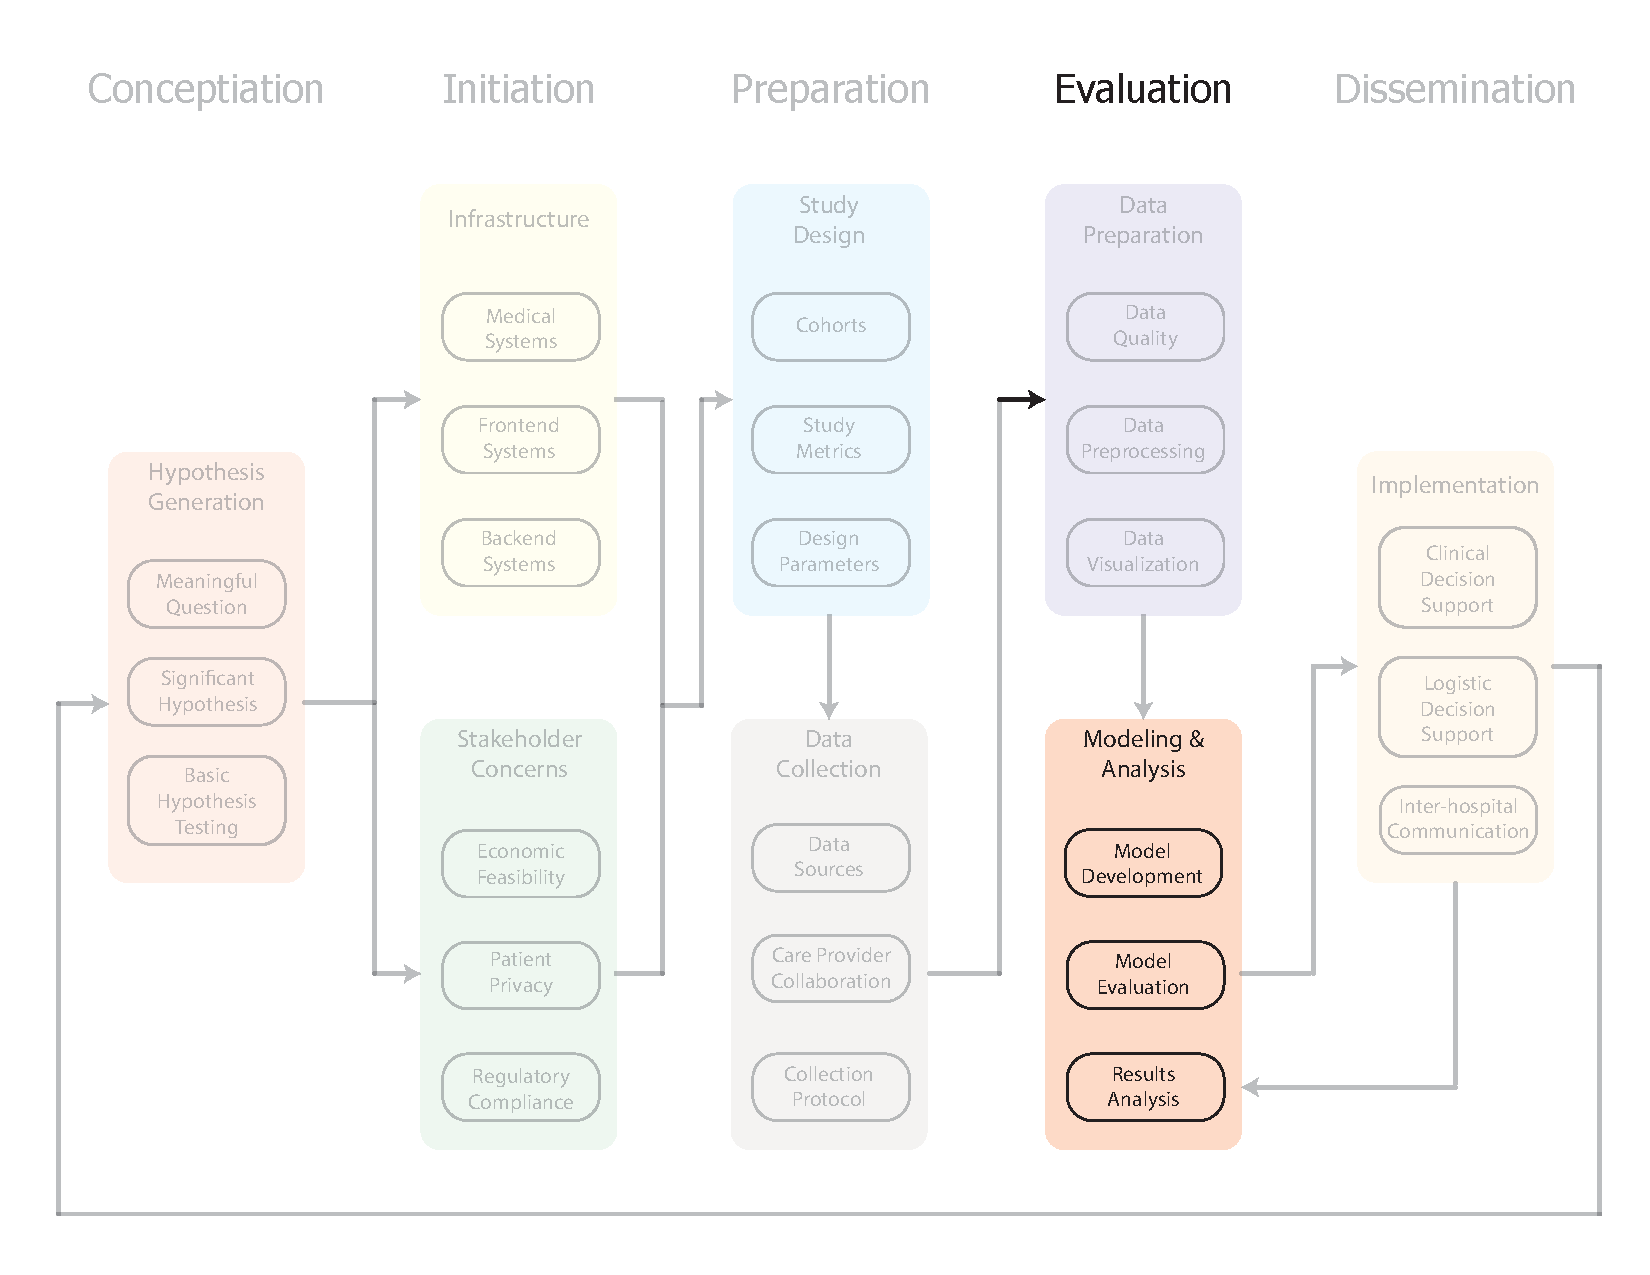
\includegraphics[width=0.8\textwidth]{images/informatics_pipeline_modeling.pdf}
	\end{center}
\end{frame}

\begin{frame}{What is Machine Learning?}
Machine Learning is part of multiple overlapping disciplines and is often associated with both Data Science and Artificial intelligence.
	\begin{center}
		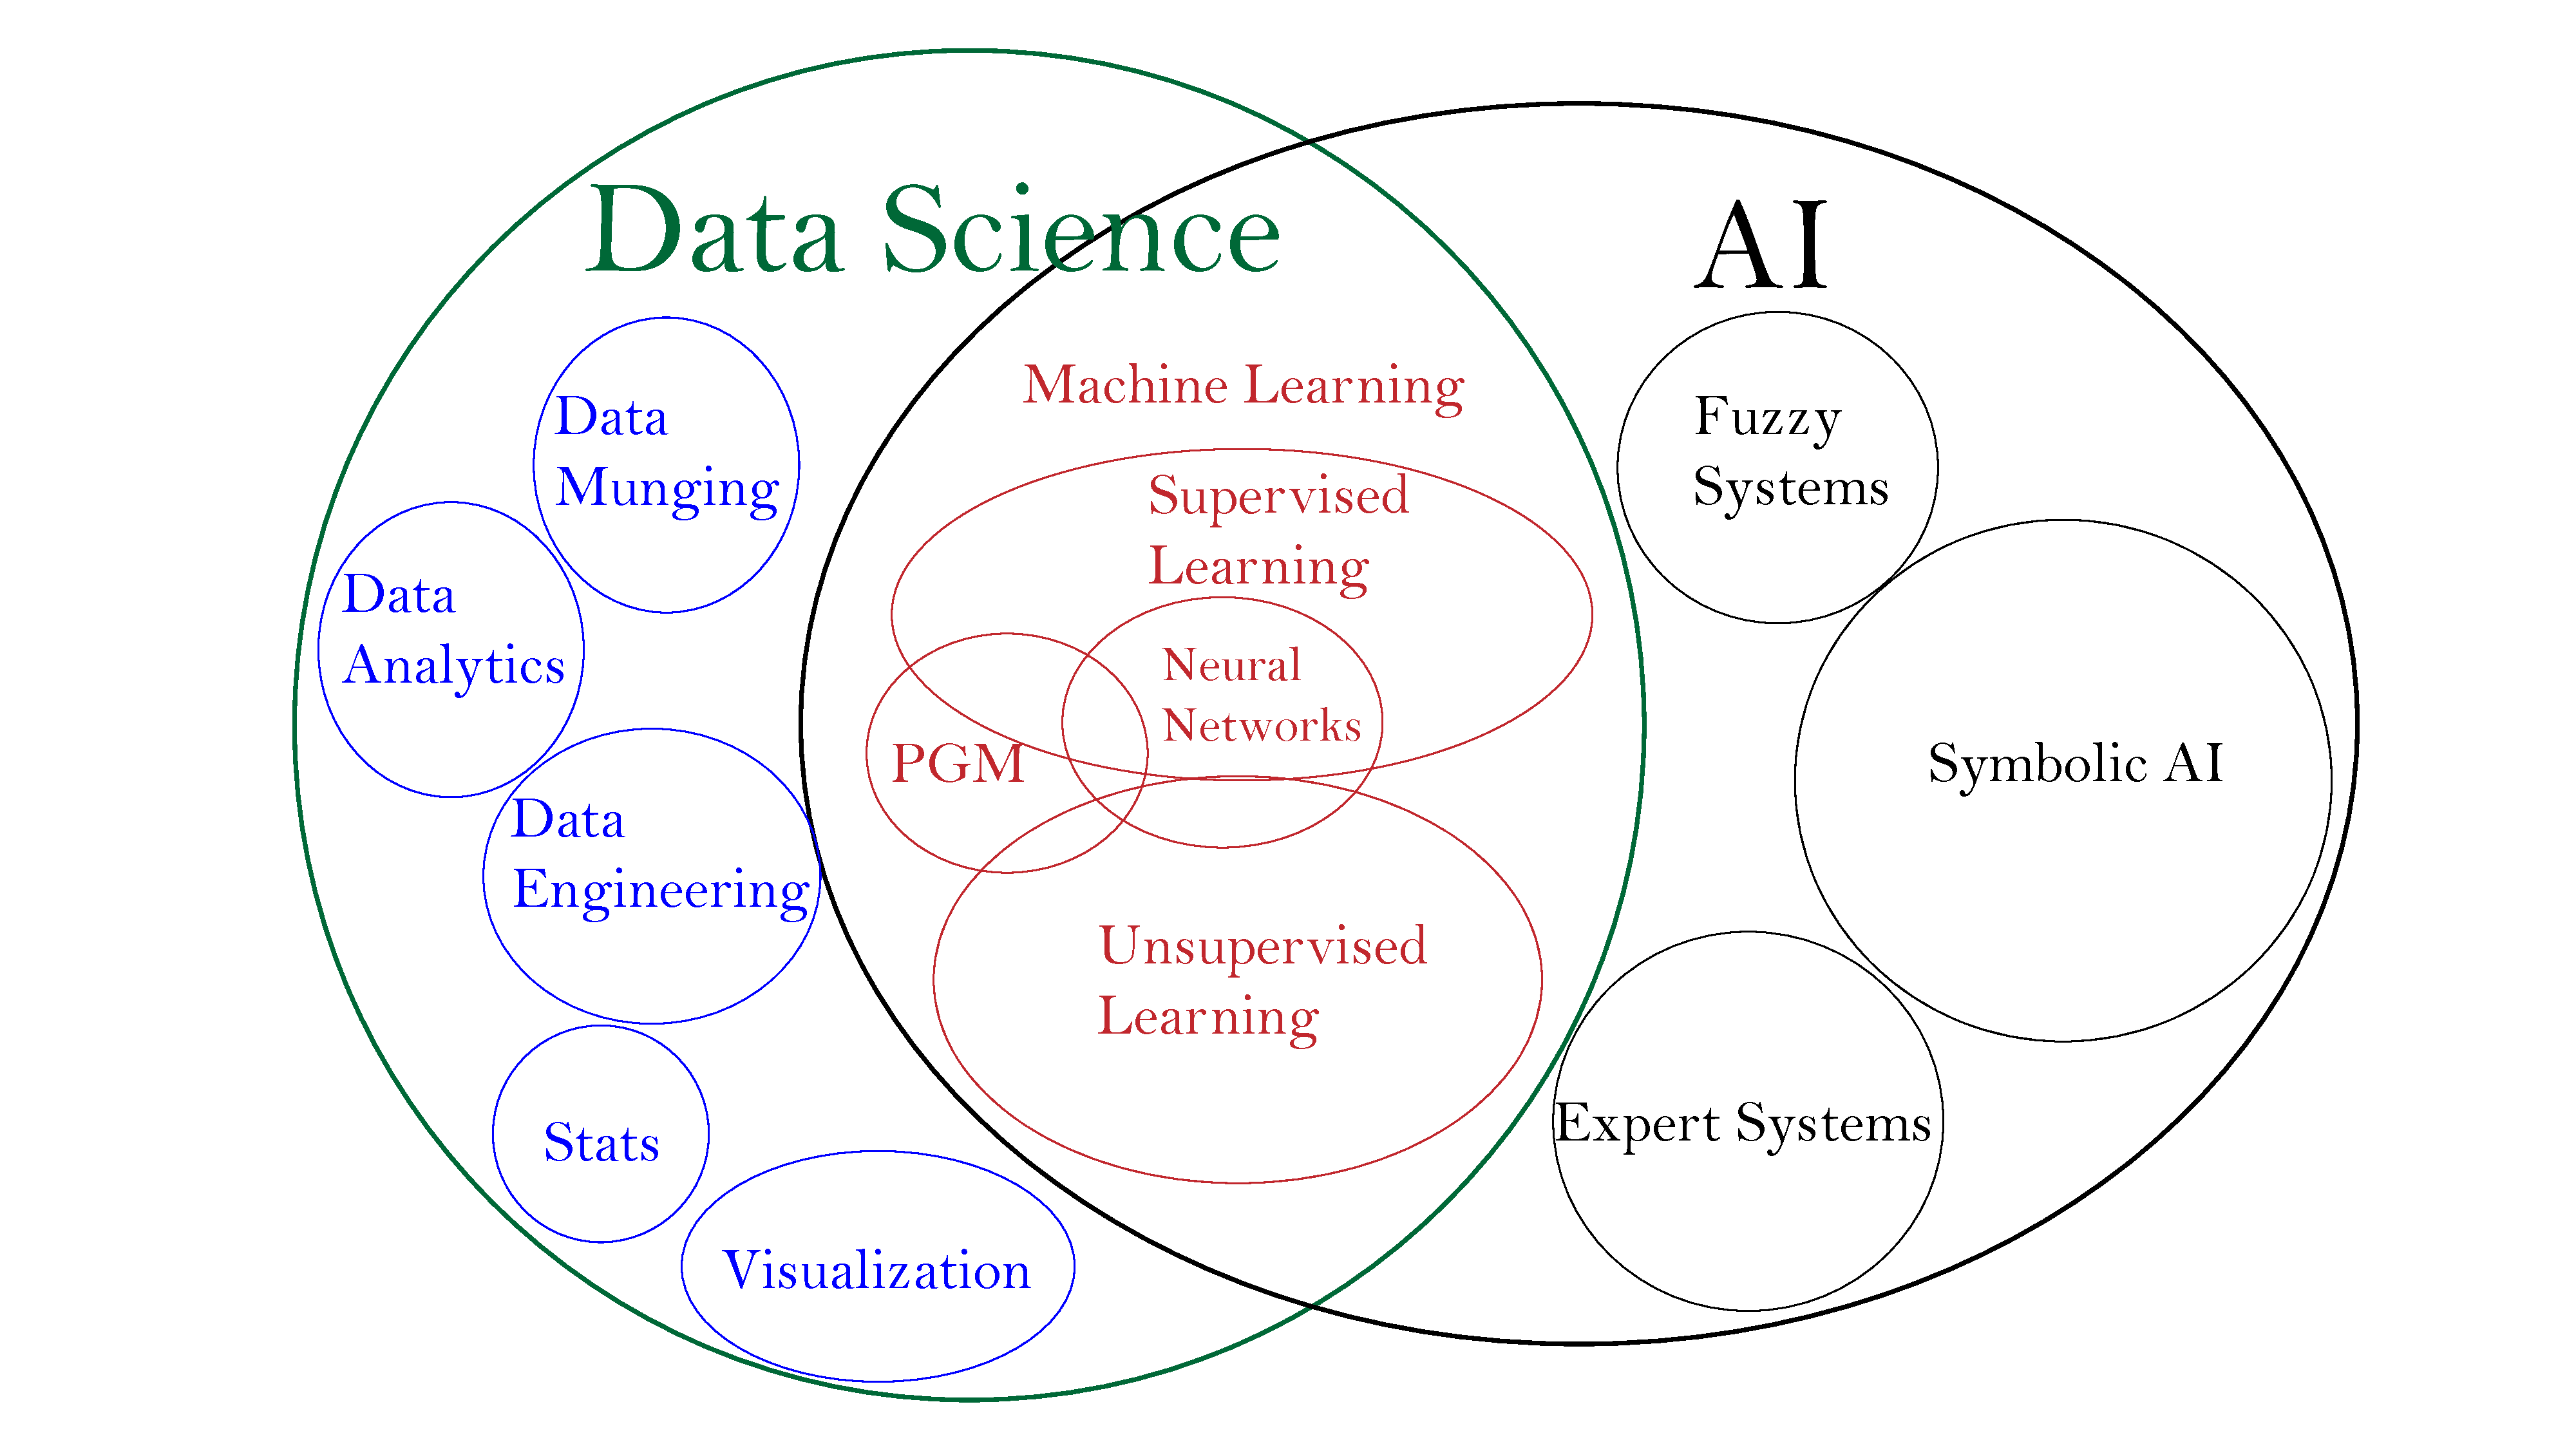
\includegraphics[width=1.2\textwidth, center, trim=-8cm -8cm 0 0cm]{images/overlapping_dis.pdf}
	\end{center}
\end{frame}

\begin{frame}{What is Machine Learning?}
\pause
	\begin{itemize}
		\item Machine learning is a discipline that uses data to improve a mathematical model
		\pause
			\begin{itemize}
				\item Algorithm Examples
					\begin{itemize}
						\item Logistic Regression
						\item Random Forest
						\item Neural Networks
					\end{itemize}
			\end{itemize}
		  \pause
		\item Machine learning contains multiple classes of learning algorithms
			\begin{itemize}
				\item Supervised Learning
				\item Unsupervised Learning
				\item Reinforcement Learning
			\end{itemize}
		  \pause
		\item Machine learning models perform tasks, such as language translation and identifying objects, that present extraordinary difficulty for standard algorithms
			\begin{itemize}
				\item ImageNet Large Scale Visual Recognition Challenge 
			\end{itemize}
		
	\end{itemize}
\end{frame}

\begin{frame}{Traditional Programming vs. Machine Learning}
	\begin{figure}
		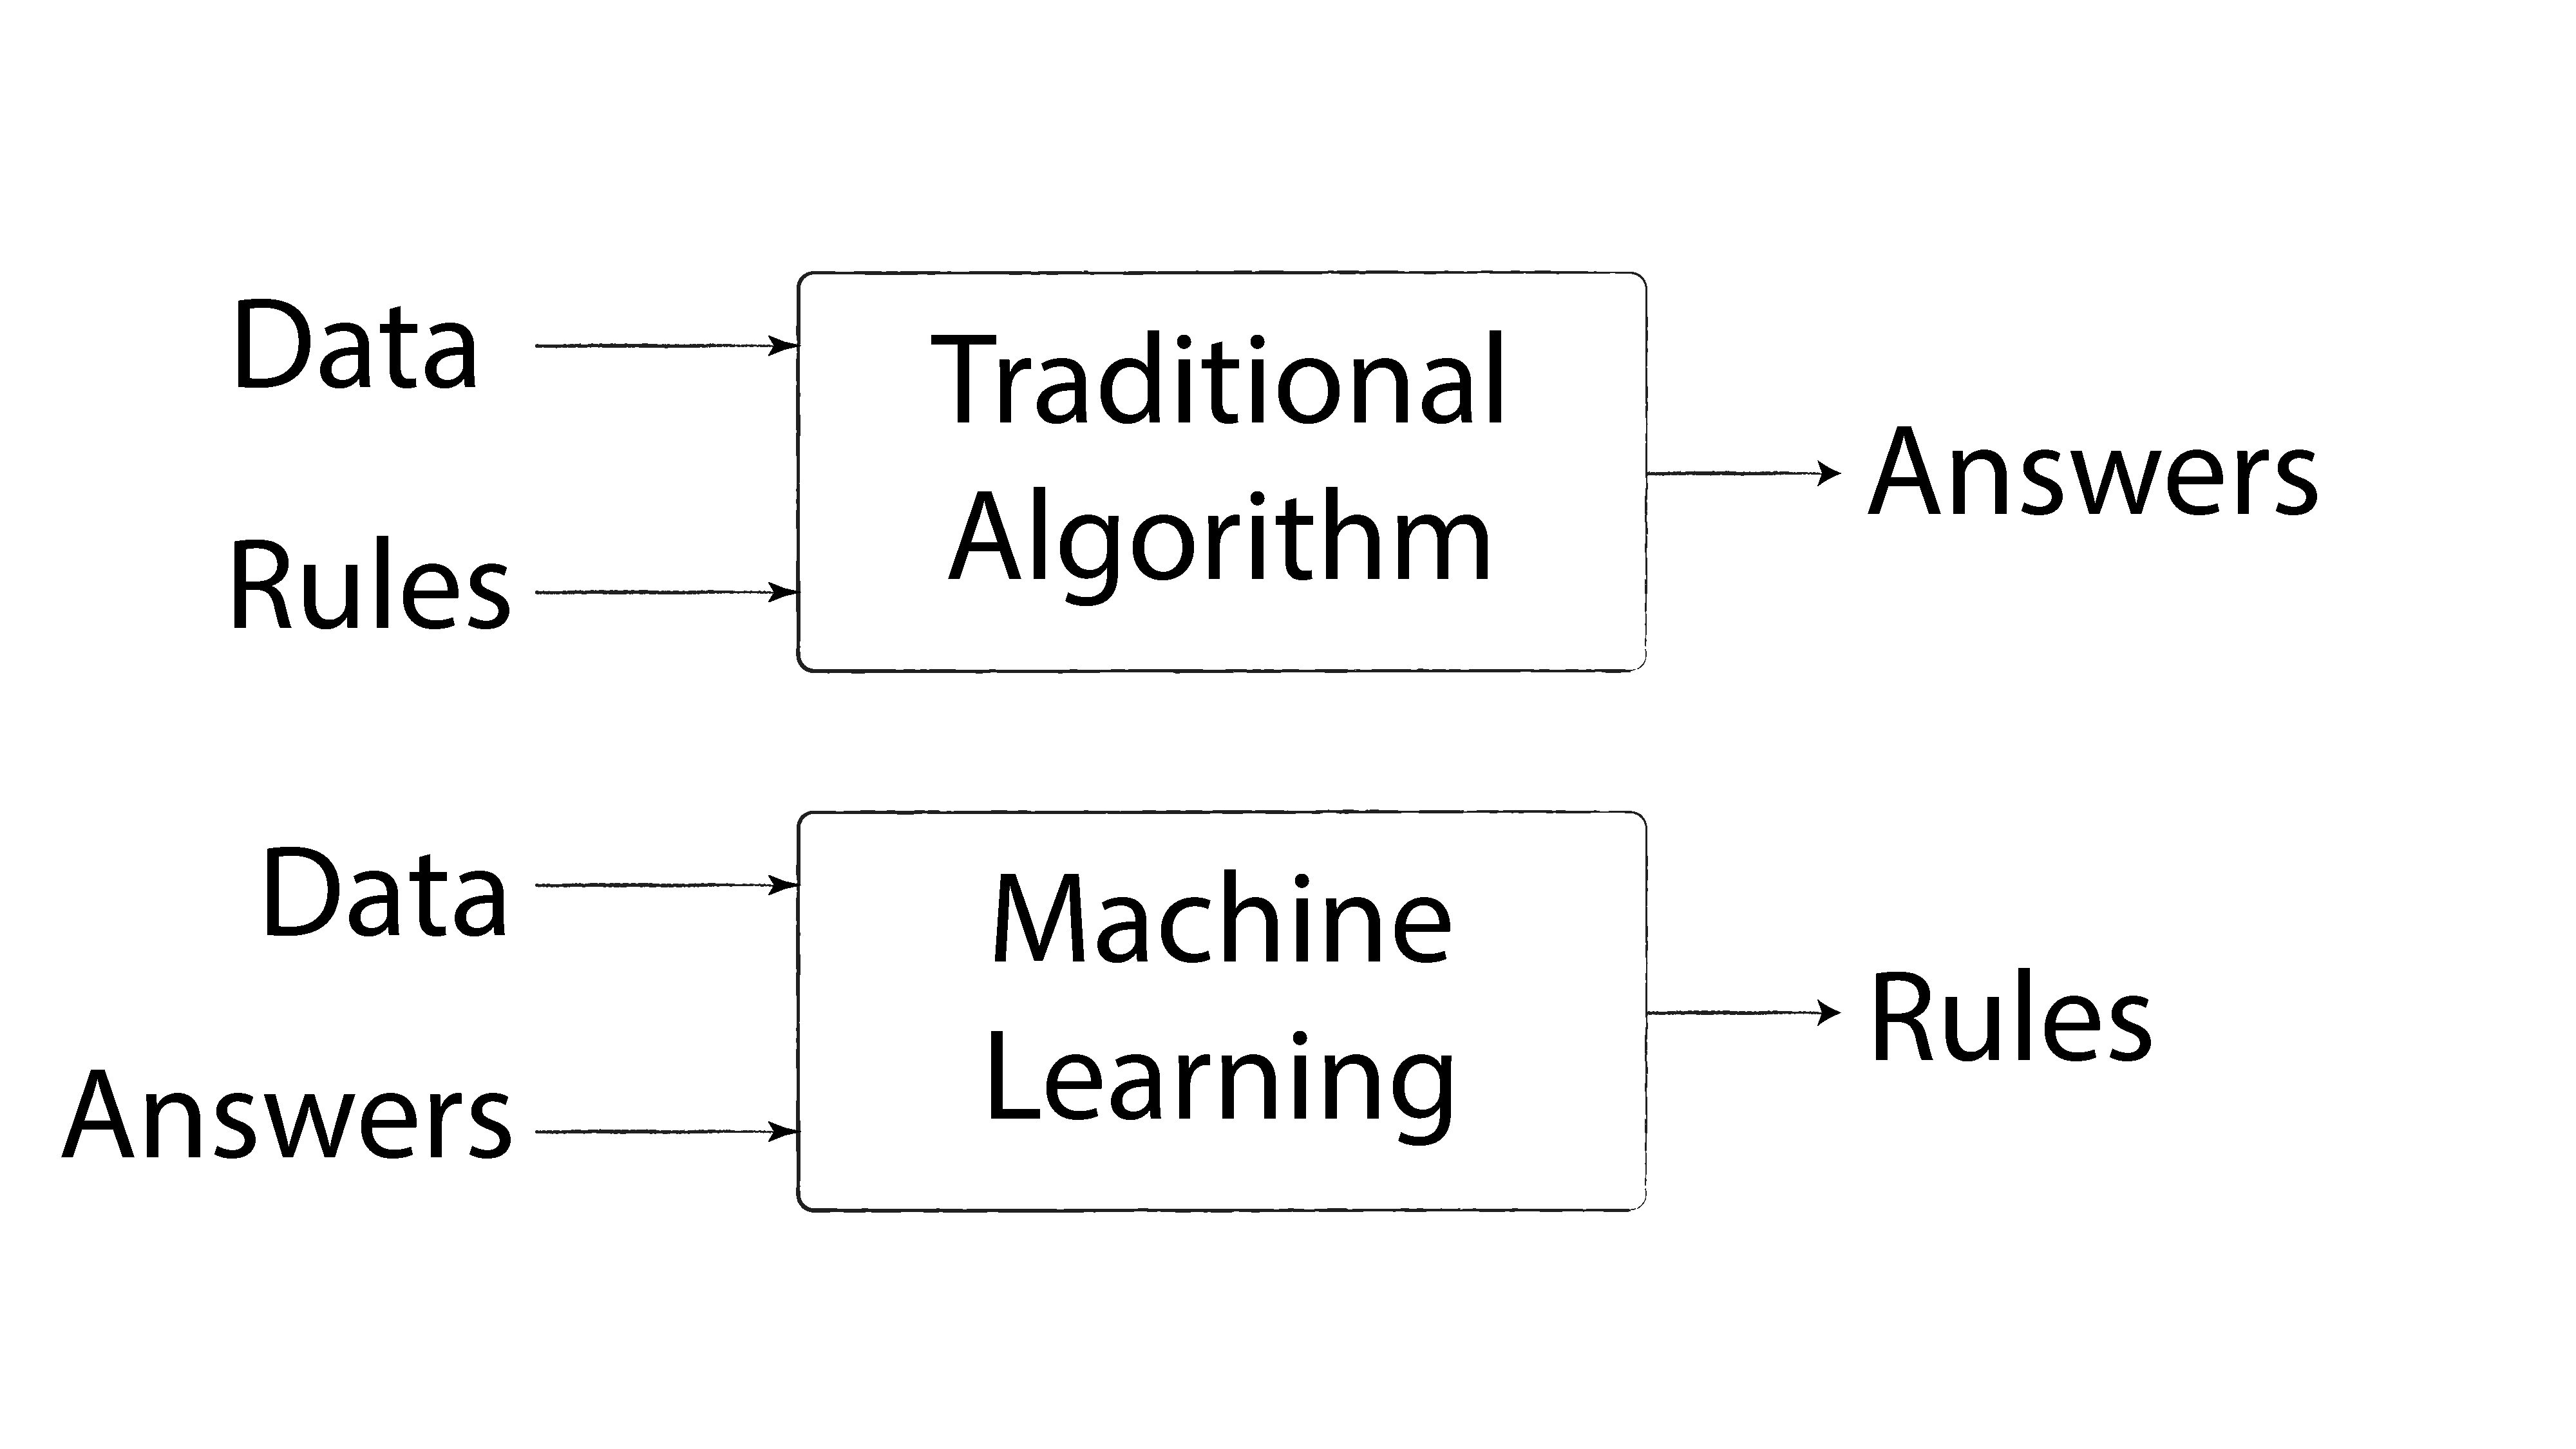
\includegraphics[width=1.0\textwidth, center, trim=0cm 0cm 0 0cm]{images/ML_paradigm.pdf}
	\end{figure}
\end{frame}

\begin{frame}{What is Machine Learning?}
Machine learning is a discipline in AI where algorithms use data to improve a model
	\begin{itemize}
		\item Algorithm is a specification of how to solve a problem
		\item Data is information about the problem we are trying to solve
		\item Model
		\begin{itemize}
			\item Scientific - a simplified and idealized understanding of physical systems
			\item Computer Science - a simulation to reproduce the behavior of a system
		\end{itemize}
	\end{itemize}
	\begin{figure}
		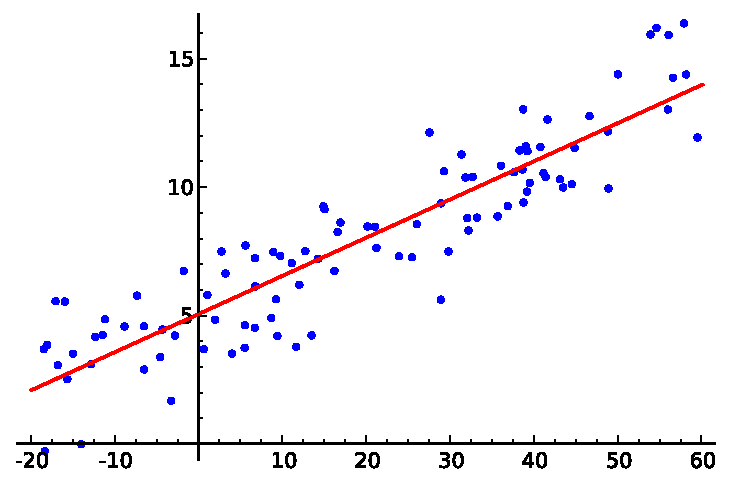
\includegraphics[width=0.5\textwidth, center, trim=0cm 0cm 0 0cm]{images/Linear_regression.pdf}
	\end{figure}
\end{frame}

\begin{frame}{Types of Learning}
	\begin{itemize}
		\item Supervised Learning
			\begin{itemize}
				\item Prediction of specific value for given data
				\begin{itemize}
					\item Algorithm learns the values (labels) from the data
					\item Learning requires the data to the desired prediction
					\item Inference is prediction of these labels from \alert{\emph{new}} data
				\end{itemize}
			\end{itemize}
		  \pause
		\item Unsupervised Learning
			\begin{itemize}
				\item Understanding the structure of the data
				\begin{itemize}
					\item Algorithm learns the structure from the data
					\item Learning/inference requires only the data
				\end{itemize}
			\end{itemize}
		  \pause
		\item Reinforcement Learning
			\begin{itemize}
				\item Predicting optimal actions for the environment based on rewards
				\begin{itemize}
					\item Algorithm learns the actions that maximize a reward for an environment 
					\item Learning requires information about the environment, rewards and actions
					\item Inference is prediction of optimal actions actions for environment
				\end{itemize}
			\end{itemize}
	\end{itemize}
\end{frame}

\begin{frame}{What is Machine Learning?}  
	\begin{itemize}
		\item ImageNet Large Scale Visual Recognition Challenge
			\begin{itemize}
				\item Algorithmic recognition of 1000 items in 150,000 photos  
			\end{itemize}
	\end{itemize}
		\begin{center}
		\begin{figure}
			\caption{ImageNet Competition Results, {\tiny By Gkrusze CC BY-SA 4.0}}
			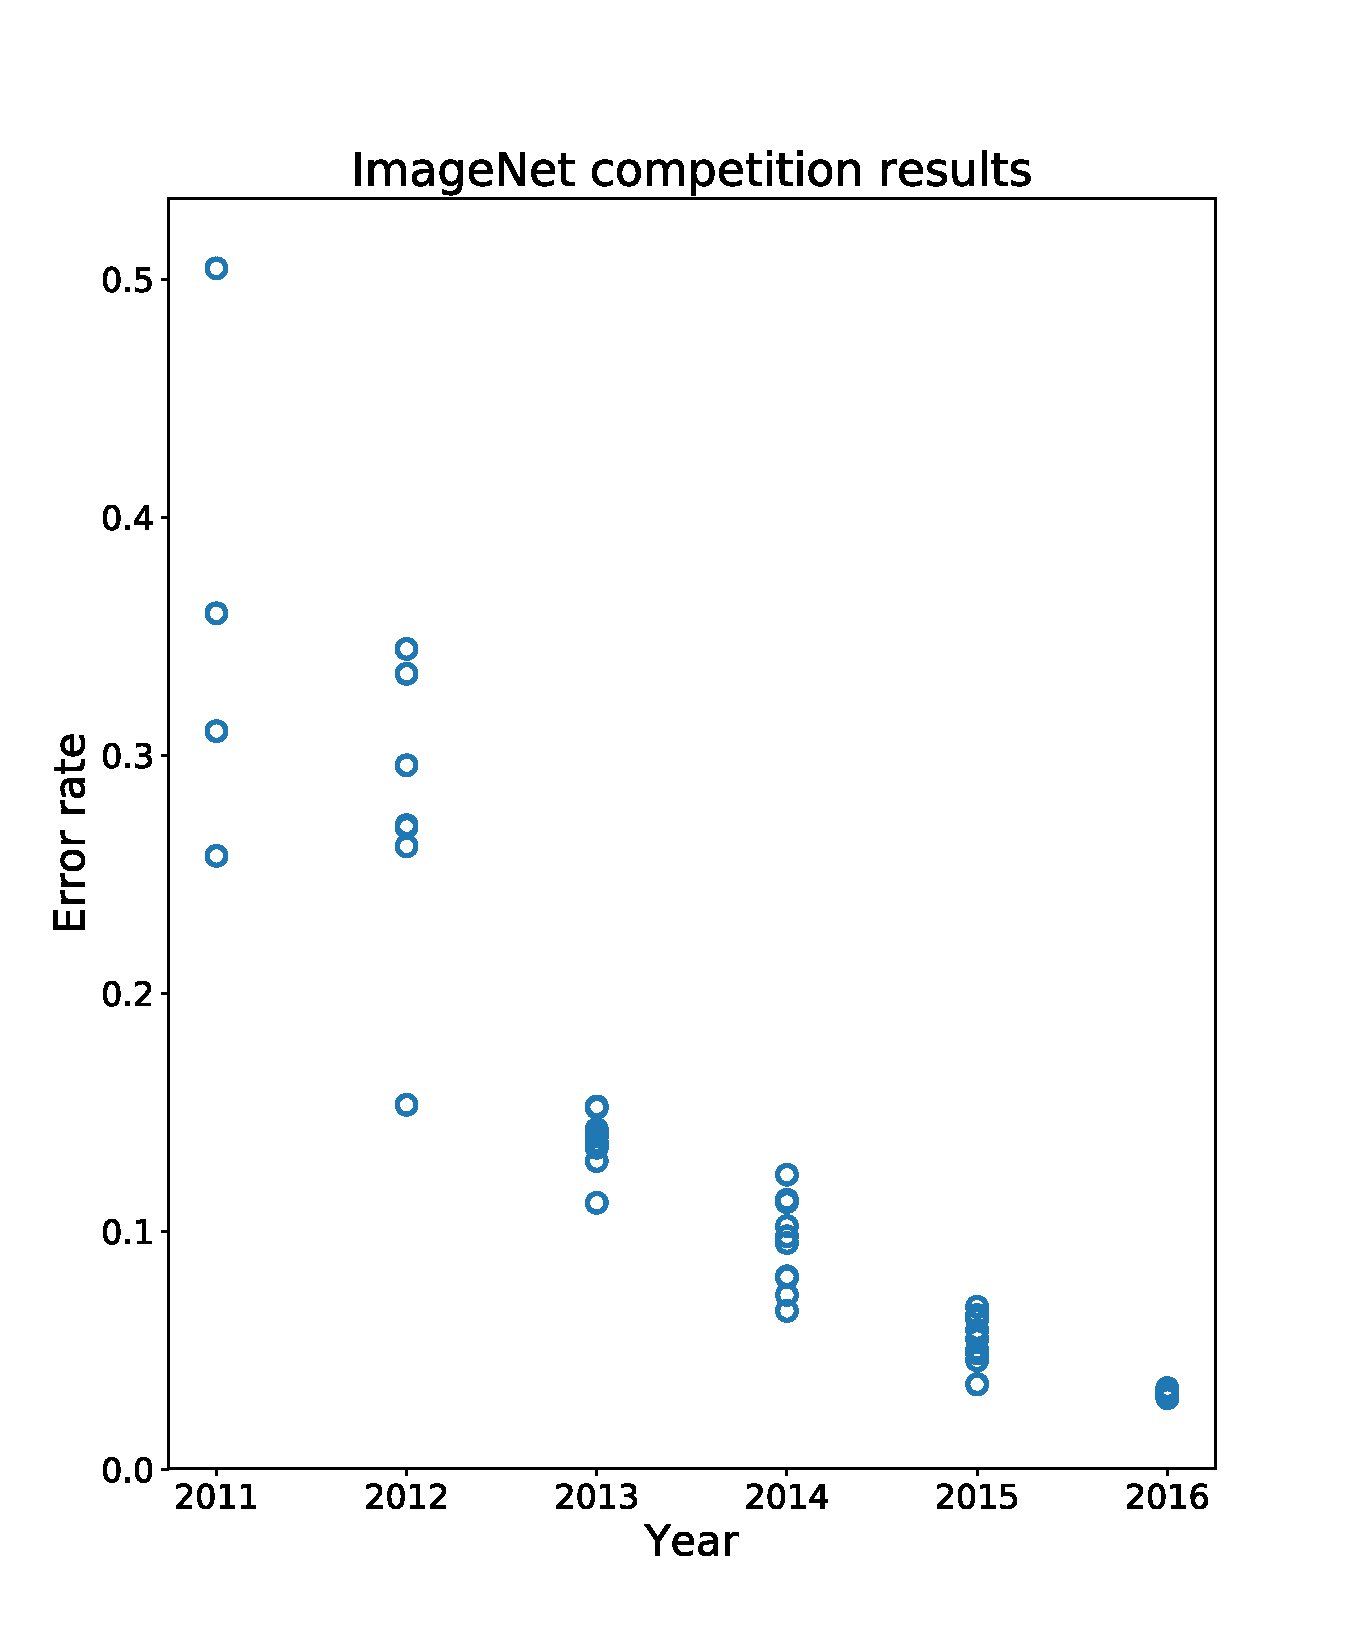
\includegraphics[width=0.45\textwidth, center, trim=0cm 0cm 0 0cm]{images/ImageNet_error.pdf}
		\end{figure}
	\end{center}
\end{frame}

\begin{frame}{What is Machine Learning?}  
	\begin{itemize}
		\item Exercise
			\begin{itemize}
				\item Using your domain expertise answer the following
				\pause
				\item Determine two problems in both Supervised and Unsupervised Learning
				\pause
				\item What types of data are required for each?
				\pause
				\item How does ML fit into the overall health care informatics pipeline?
				\pause
				\item How can you used both in a single project?
			\end{itemize}
	\end{itemize}
\end{frame}

\section{Supervised Learning}

\subsection{Supervised Prediction Types}

\begin{frame}{Types of Supervised Learning}
\emph{What are the type of supervised learning?}
	\begin{itemize}
		\item Regression - predicting a continuous numerical value
		\pause
		\item Classification - prediction of discreet class labels
		\pause
	\end{itemize}
	\begin{columns}
	\begin{column}{0.5\textwidth}
	\begin{figure}	
		\caption{Non-linear Regression, {\tiny By Alexeicolin - Own work, CC BY-SA 3.0}}
		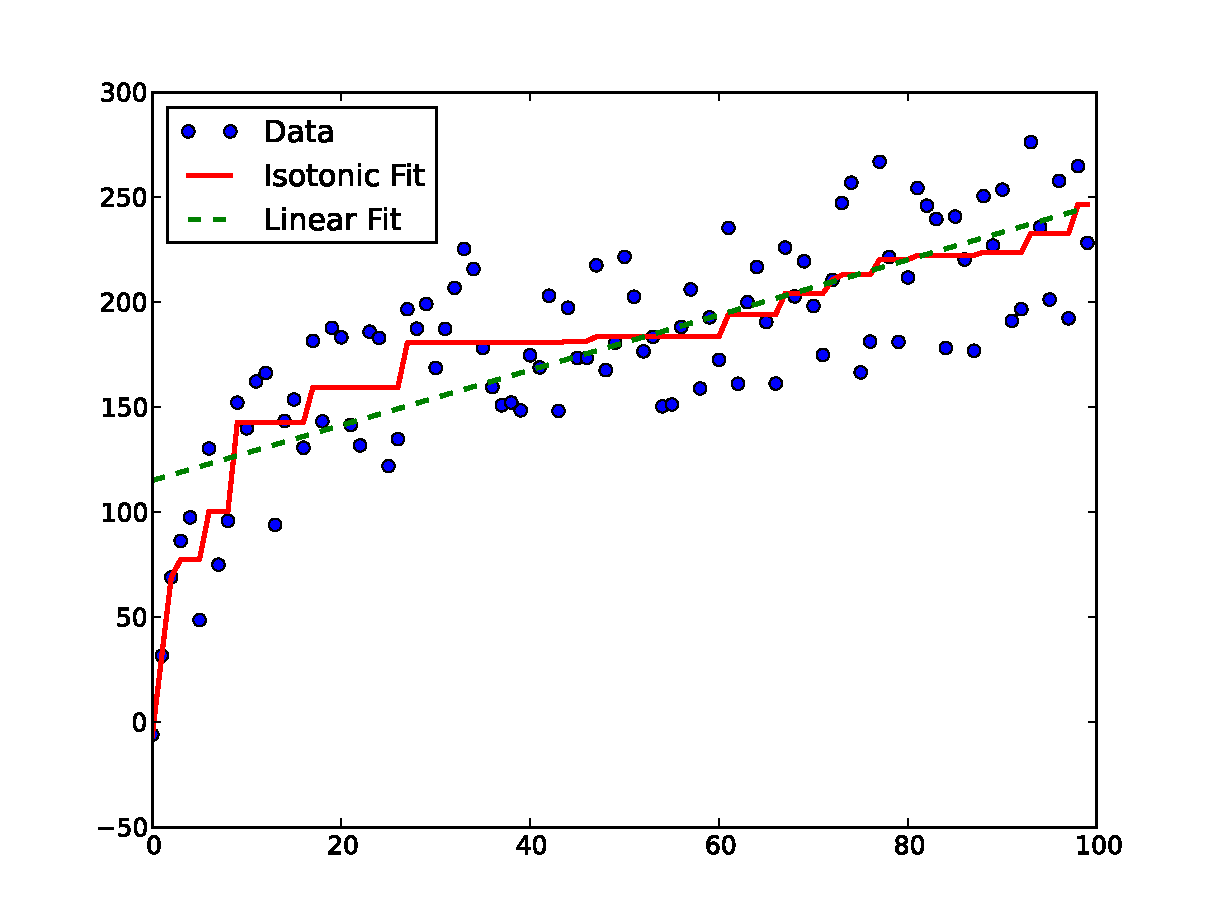
\includegraphics[width=0.9\textwidth, center, trim=0cm 0cm 0 0cm]{images/Isotonic_regression.pdf}
	\end{figure}
	\end{column}
	\begin{column}{0.5\textwidth}
		\begin{figure}	
		\caption{Classification, {\tiny By Alisneaky Own work, CC BY-SA 4.0}}
		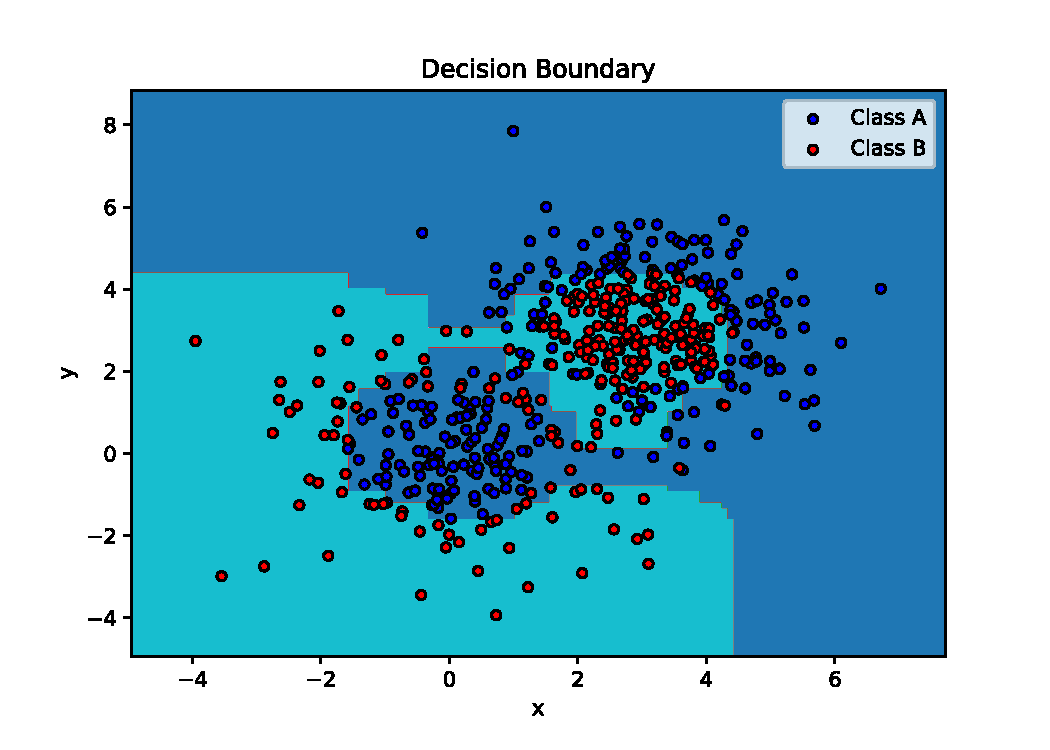
\includegraphics[width=0.9\textwidth, center, trim=0cm 0cm 0 0cm]{images/Classification.pdf}
	\end{figure}
	\end{column}
	\end{columns}
\end{frame}

\begin{frame}{Types of Predictions}  
	\begin{itemize}
		\item Exercise
			\begin{itemize}
				\item Determine the types of predictions for the Supervised Learning problem above
				\pause
				\item How many classes do the Classifications problems have?
			\end{itemize}
	\end{itemize}
\end{frame}

\subsection{Basic Methods}

\begin{frame}{Basic Methods}
\emph{Linear and Logistic Regression}
	\begin{itemize}
		\item Linear Regression - Predicting continuous values from linearly separable data
		\pause
		\item Logistic Regression - Subclass of Generalized Linear Models for binary class prediction
	   \pause
       \item \emph{Data \alert{should} be linearly separable or variables linearly correlated}
	\end{itemize}
\end{frame}

\begin{frame}{Linear Regression}
Predicting continuous values
	\begin{figure}	
		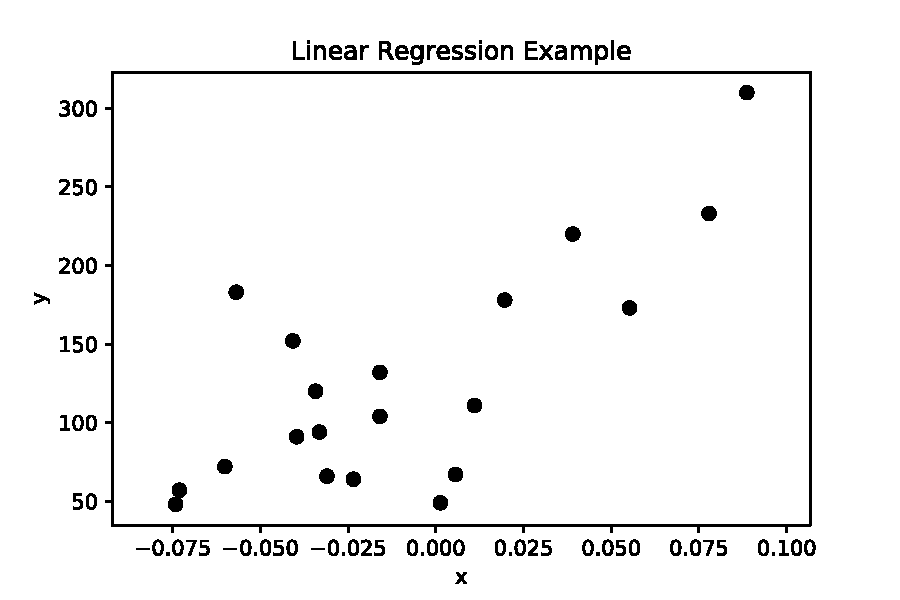
\includegraphics[width=0.9\textwidth, center, trim=0cm 0cm 0 0cm]{images/Linear_scatter.pdf}
	\end{figure}
\end{frame}

\begin{frame}{Linear Regression}
Predicting continuous values
	\begin{figure}	
		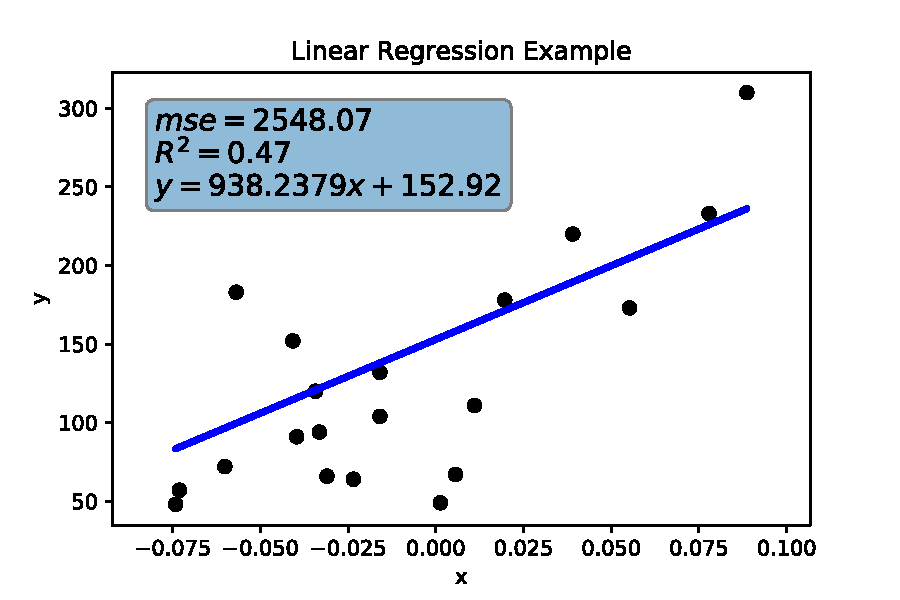
\includegraphics[width=0.9\textwidth, center, trim=0cm 0cm 0 0cm]{images/Linear_Reg_scatter.pdf}
	\end{figure}
\end{frame}

\begin{frame}{Logistic Regression}
What if the data is binary?
	\begin{figure}	
		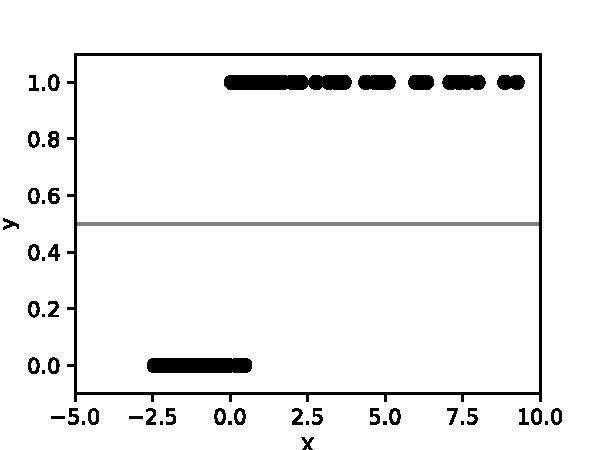
\includegraphics[width=0.9\textwidth, center, trim=0cm 0cm 0 0cm]{images/logit_data.pdf}
	\end{figure}
\end{frame}

\begin{frame}{Logistic Regression}
The linear fit does not work
	\begin{figure}	
		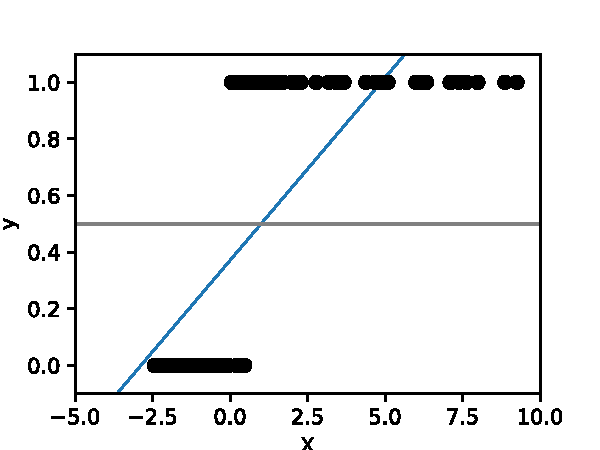
\includegraphics[width=0.9\textwidth, center, trim=0cm 0cm 0 0cm]{images/logit_line_data.pdf}
	\end{figure}
\end{frame}

\begin{frame}{Logistic Regression}
Sigmoid function fits the data well 
	\begin{figure}	
		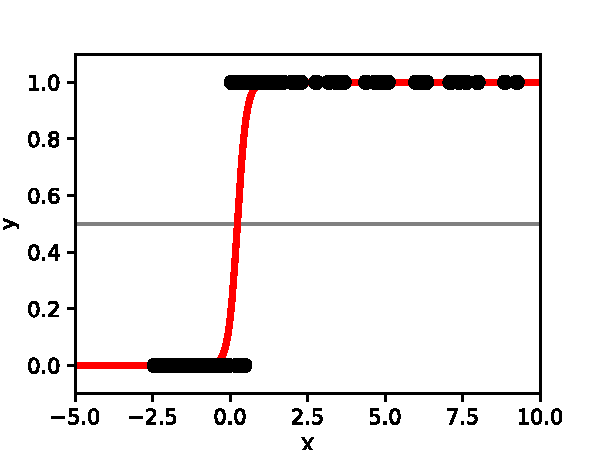
\includegraphics[width=0.9\textwidth, center, trim=0cm 0cm 0 0cm]{images/logit_curve_data.pdf}
	\end{figure}
\end{frame}

\begin{frame}{Logistic Regression}
Logistic regression fits uses a linear fit to a sigmoid function
	\begin{figure}	
		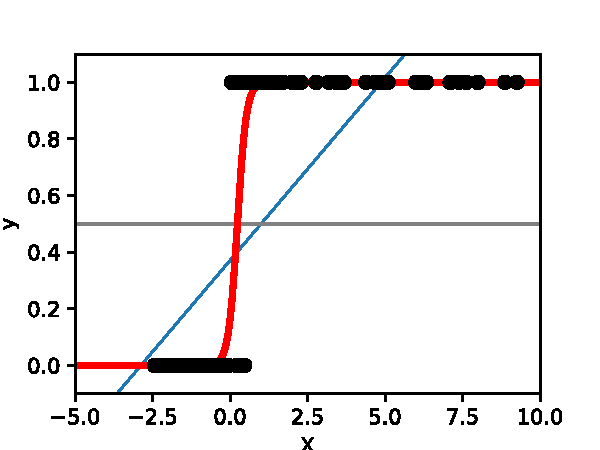
\includegraphics[width=0.9\textwidth, center, trim=0cm 0cm 0 0cm]{images/logit_curve_line_data.pdf}
	\end{figure}
\end{frame}

\subsection{SVM and Tree-Based Methods}

\begin{frame}{Iris Data}
\emph{The iris data set is commonly used for teaching machine learning}
	\begin{columns}
	\begin{column}{0.5\textwidth}
	\begin{itemize}
		\item Data from 1930's to identify flowers from petal and sepal measurements
		\item Three species of iris flowers: Setosa, Versicolor and Virginica
		\item Only a few variables, Sepal width, Sepal length, Petal width and Petal length
		\item 150 sets of measurements 
	\end{itemize}
	\end{column}
	\begin{column}{0.5\textwidth}
		\begin{figure}	
			\caption{Versicolor Iris flower, sepal labeled}
			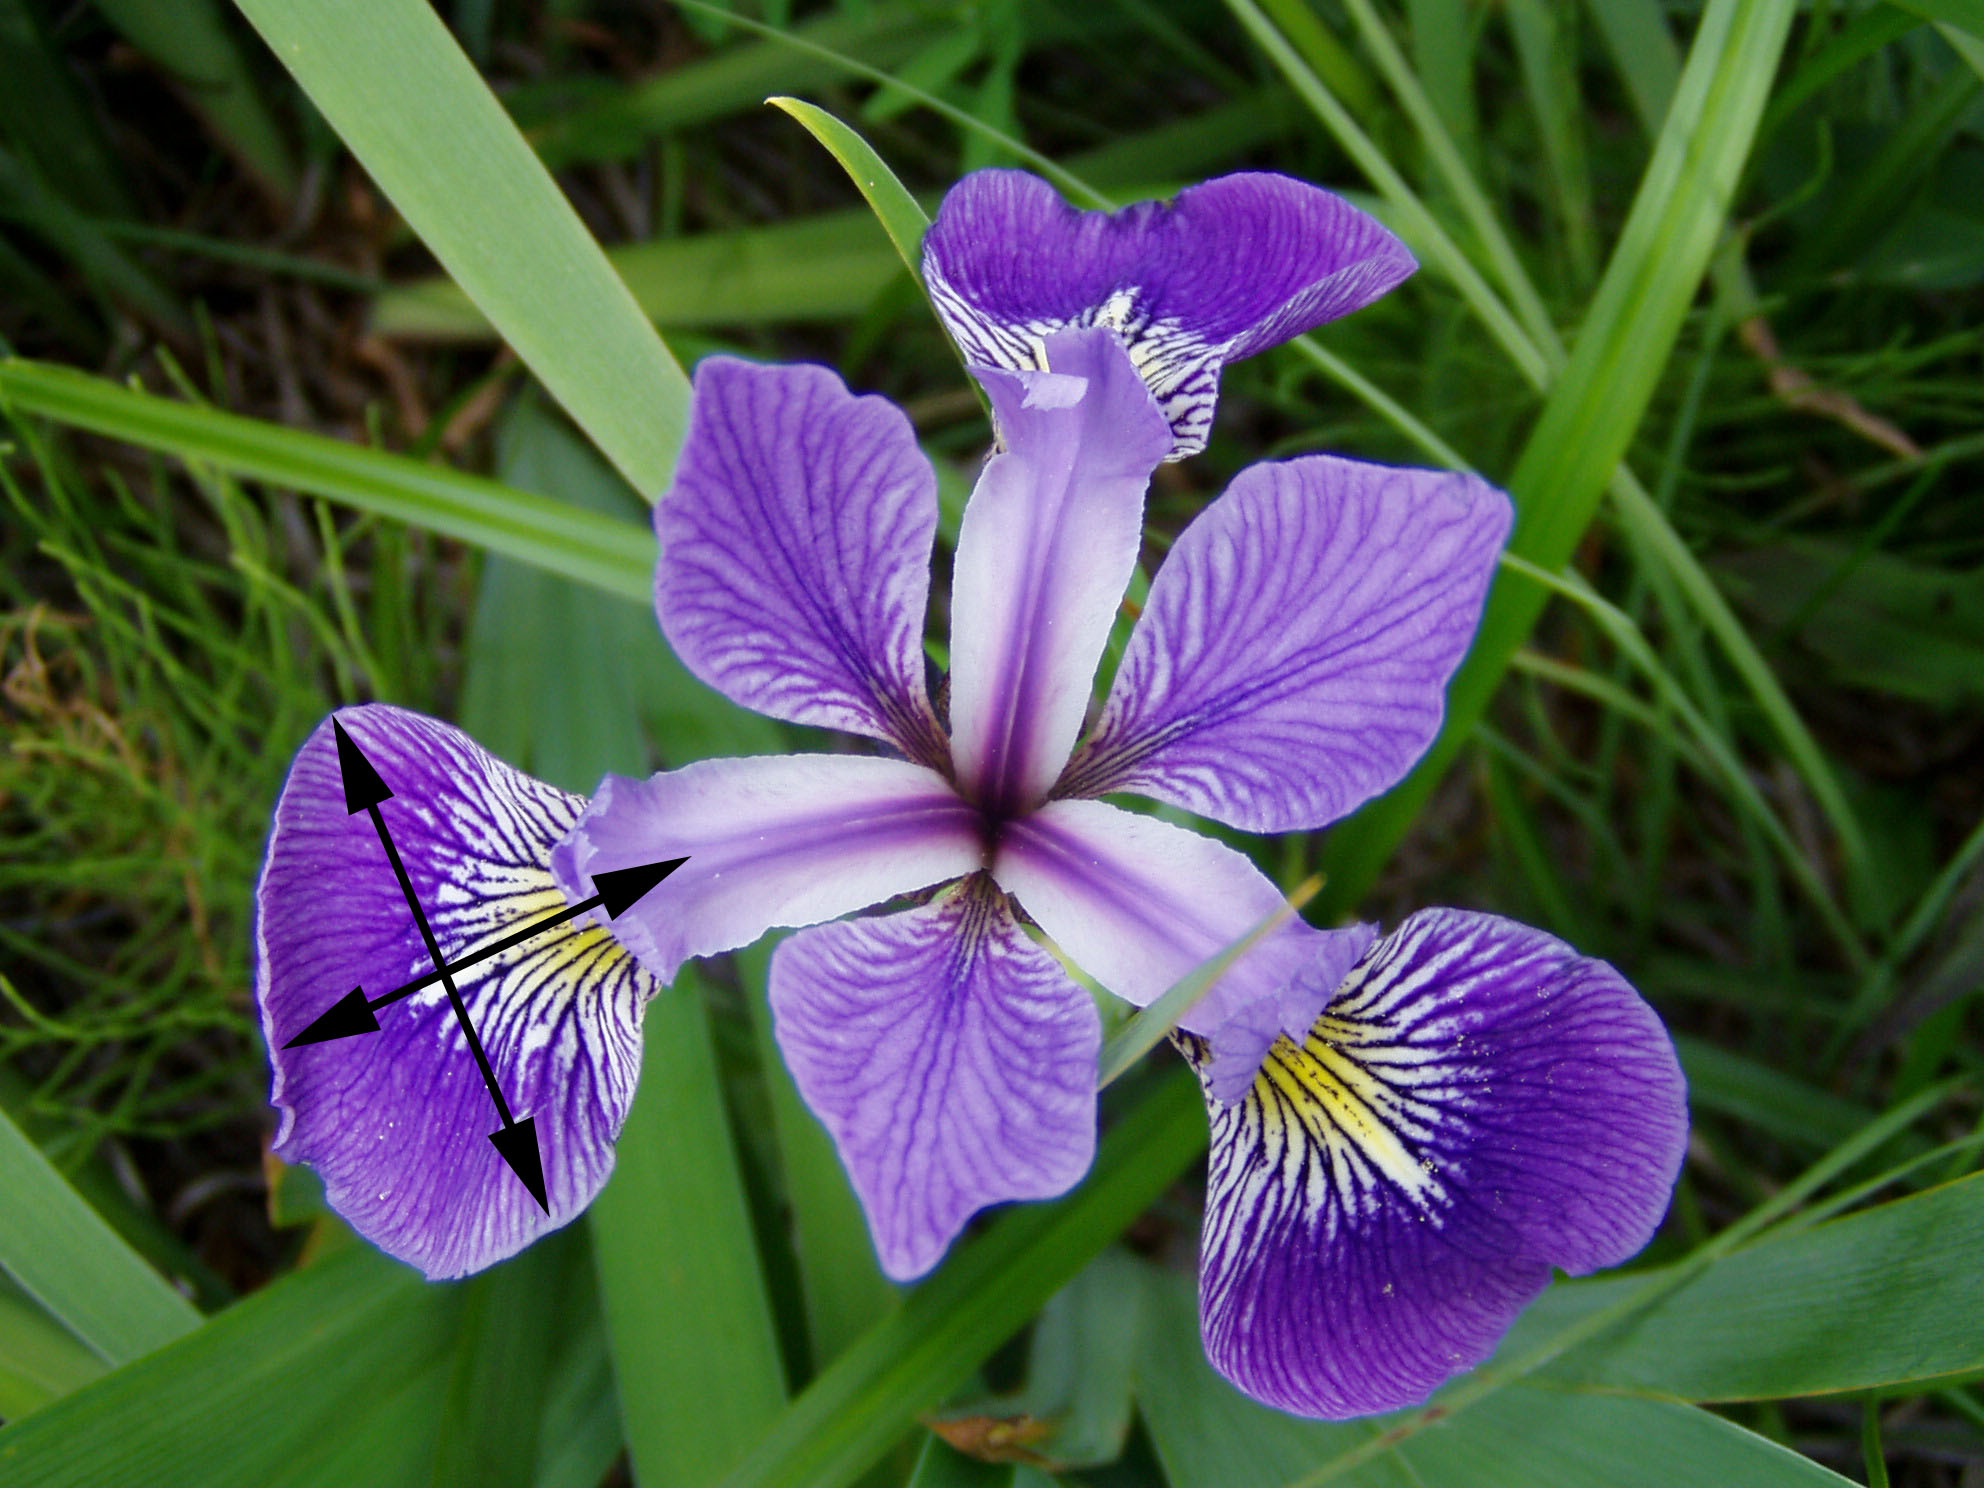
\includegraphics[width=1.0\textwidth, center, trim=0cm 0cm 0 0cm]{images/Iris_versicolor_arrows.jpg}
	\end{figure}
	\end{column}
	\end{columns}
\end{frame}

\begin{frame}{Iris Data}
Dataset of Iris Flower Types
	\begin{figure}	
		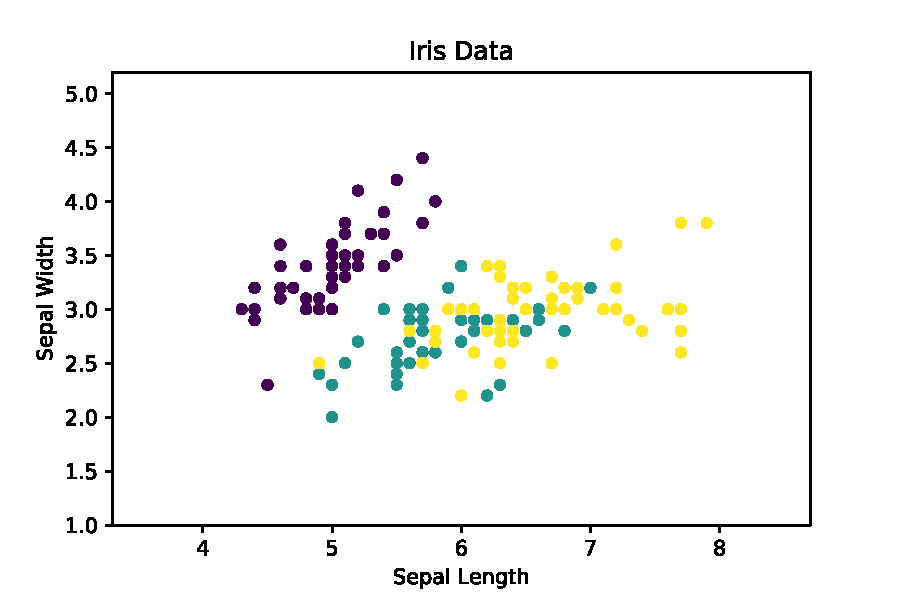
\includegraphics[width=0.9\textwidth, center, trim=0cm 0cm 0 0cm]{images/Iris_Data.pdf}
	\end{figure}
\end{frame}

\begin{frame}{Non-parametric Methods}
\emph{Support Vector Machines and Decision Trees}
	\begin{itemize}
		\item Support Vector Machine - Prediction by finding the best (hyper)planes that separate the data 
		\item Tree-Based Method - Prediction of using decision-trees
		\begin{itemize}
			\item Decision Trees
			\item Random Forest
			\item Boosted Trees
		\end{itemize}
	\end{itemize}
\end{frame}

\begin{frame}{Support Vector Machines}
\emph{SVC and SVR are a common methods of fitting data}
	\begin{columns}
	\begin{column}{0.5\textwidth}
	\begin{itemize}
		\item Finds the plane that \emph{best} divides the data
		\item Can fit highly non-linear data
		\item Kernels allow for flexibility but must be chosen by the user
		\item Does not fit data with more than two classes
		\item Does not give class probabilities just class membership
		\item Parameters can be difficult to choose
	\end{itemize}
	\end{column}
	\begin{column}{0.5\textwidth}
		\begin{figure}	
			\caption{Best plane example, {\tiny By User:ZackWeinberg, based on PNG by User:Cyc derived from: Svm separating hyperplanes.png, CC BY-SA 3.0}}
			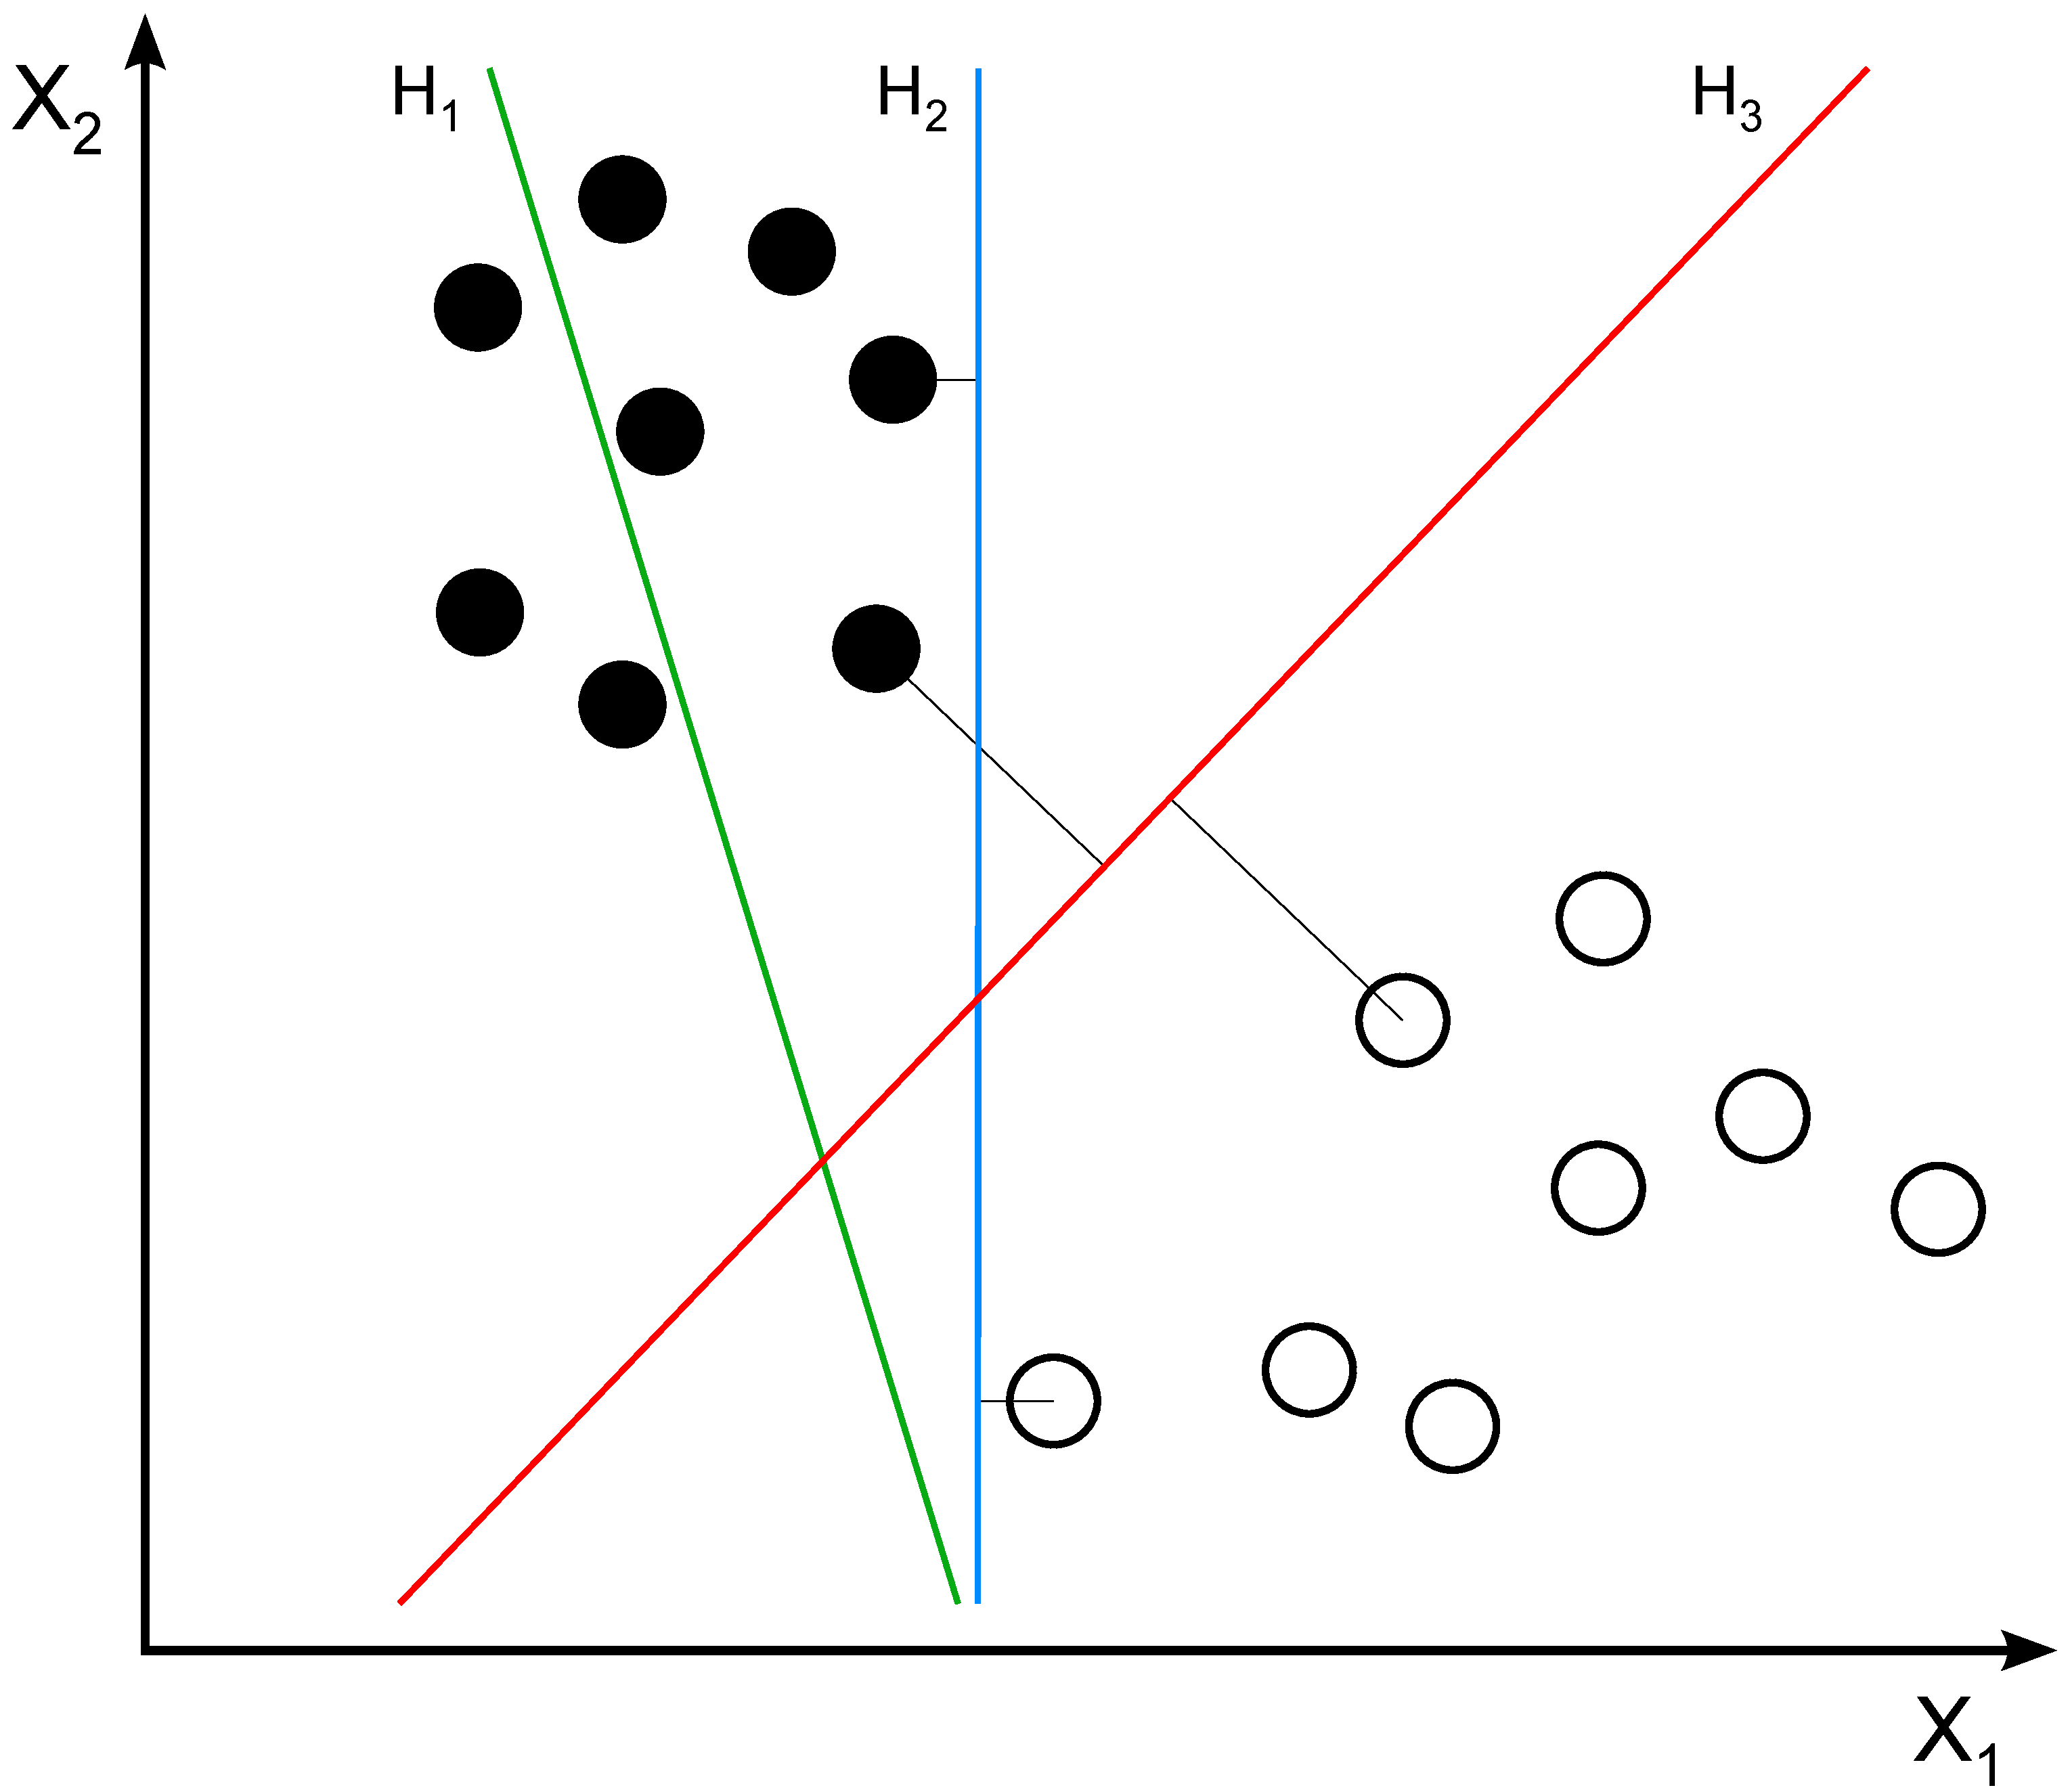
\includegraphics[width=1.0\textwidth, center, trim=0cm 0cm 0 0cm]{images/Svm_separating_hyperplanes.pdf}
	\end{figure}
	\end{column}
	\end{columns}
\end{frame}


\begin{frame}{Support Vector Machine}
	\begin{figure}	
		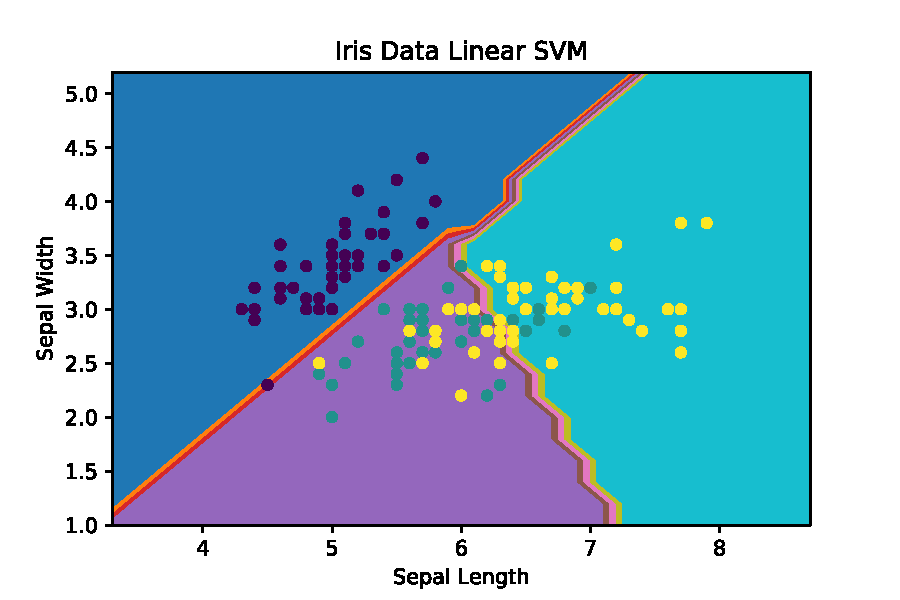
\includegraphics[width=0.9\textwidth, center, trim=0cm 0cm 0 0cm]{images/Iris_Data_labeled_linear.pdf}
	\end{figure}
\end{frame}

\begin{frame}{Support Vector Machine}
	\begin{figure}	
		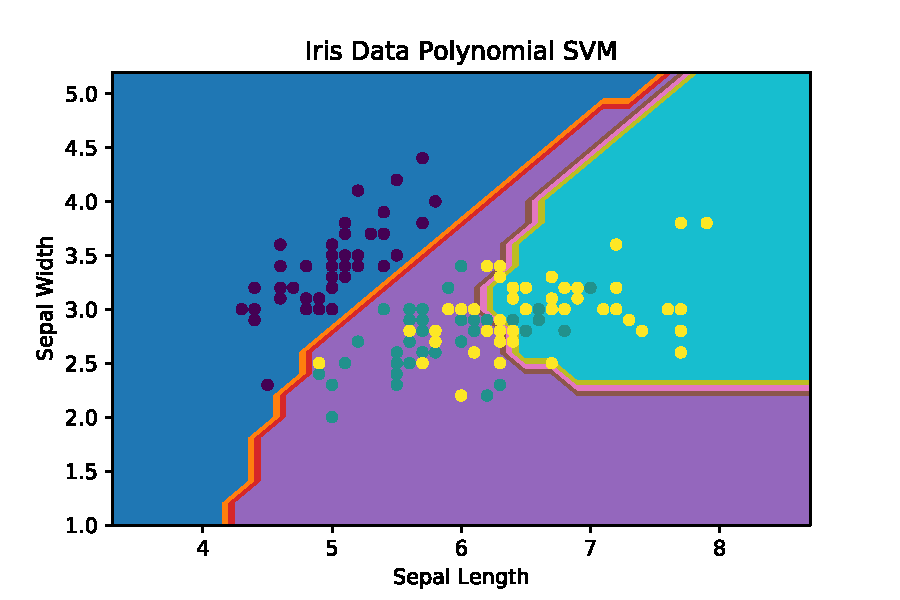
\includegraphics[width=0.9\textwidth, center, trim=0cm 0cm 0 0cm]{images/Iris_Data_labeled_poly.pdf}
	\end{figure}
\end{frame}

\begin{frame}{Tree-based Methods}
\emph{Methods using decision trees or ensembles of decision trees for classification and regression problems}
	\begin{columns}
	\begin{column}{0.5\textwidth}
	\begin{itemize}
		\item Fits a decision tree based on the data to predict results
		\item Can fit highly non-linear data with \emph{high} accuracy
		\item Models can be very large
		\item Some models, Random Forest, do not fit sparse data well
		\item Other models, Boosting, have many parameters that can be difficult to choose
	\end{itemize}
	\end{column}
	\begin{column}{0.5\textwidth}
		\begin{figure}
			\caption{Decision Tree Example}
			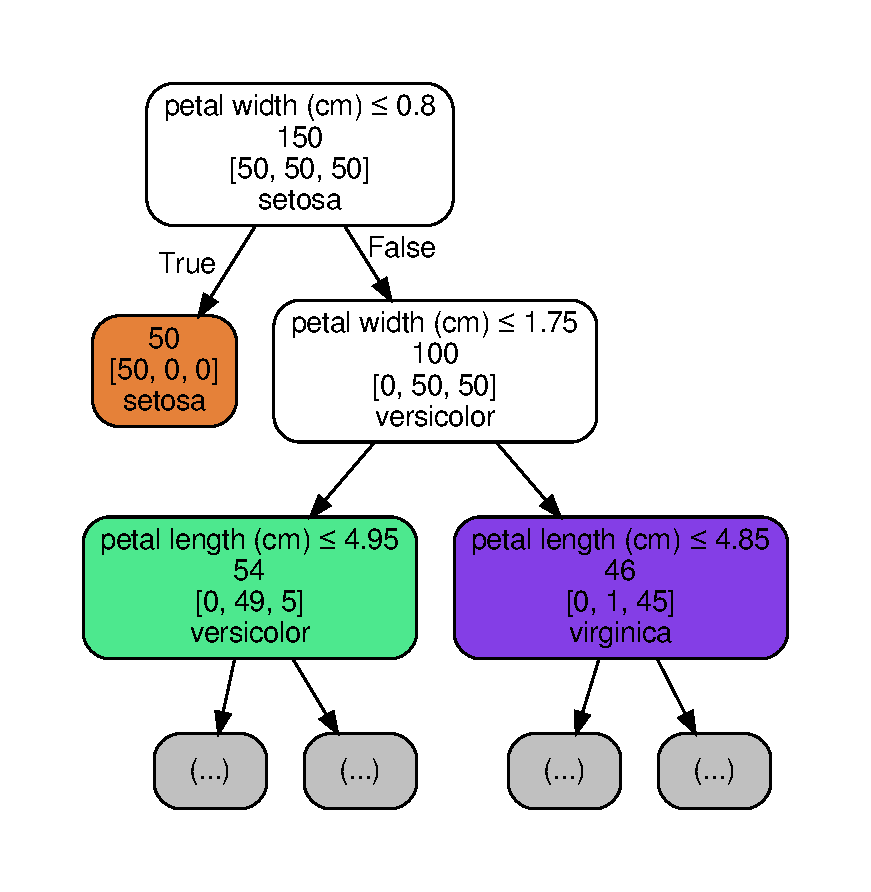
\includegraphics[width=1.0\textwidth, center, trim=1cm 0cm 0 0cm]{images/DT_3_simple.pdf}
	\end{figure}
	\end{column}
	\end{columns}
\end{frame}

\begin{frame}{Building a Decision Tree}
Make splits in the data in such a way that it separates the classes or that minimizes the distance between the predictions in a region.
		\begin{figure}	
			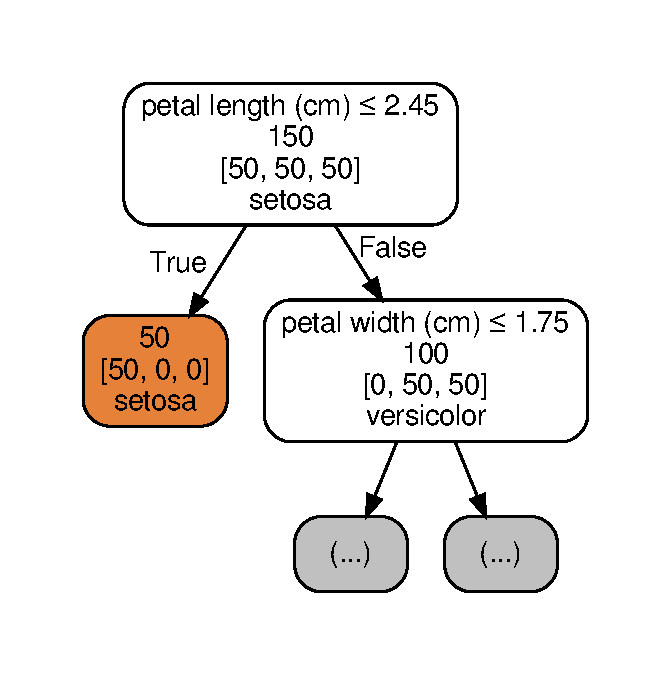
\includegraphics[width=0.55\textwidth, center, trim=0cm 0cm 0 0cm]{images/DT_2_simple.pdf}
	\end{figure}
\end{frame}

\begin{frame}{Building a Decision Tree}
		\begin{figure}	
			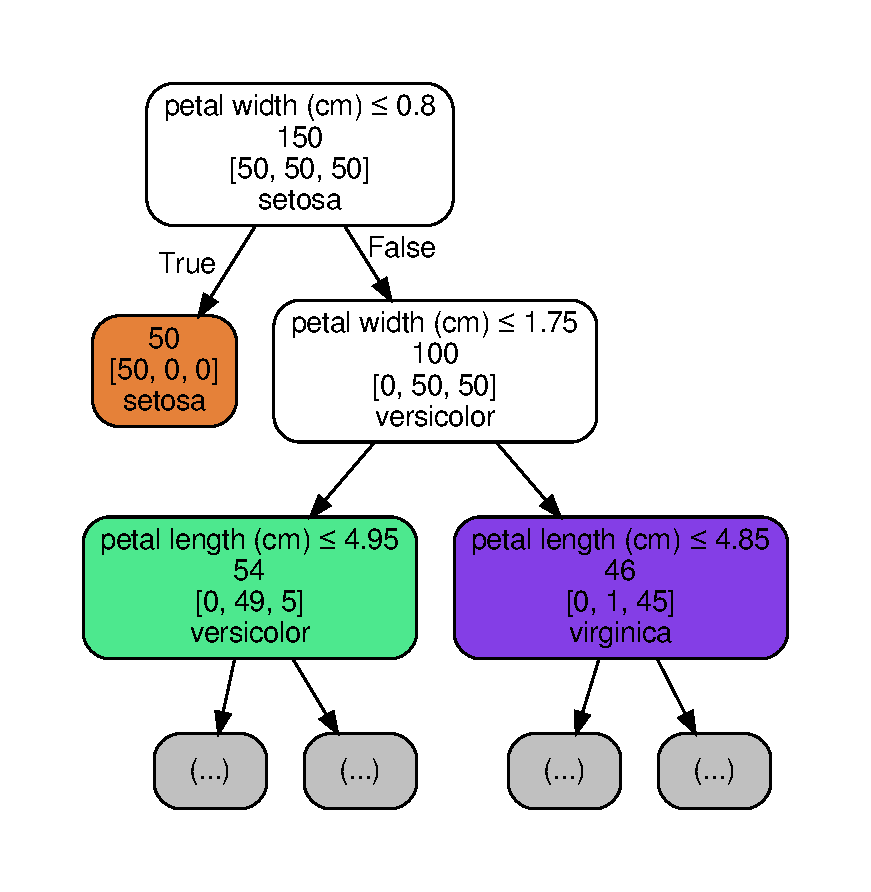
\includegraphics[width=0.75\textwidth, center, trim=0cm 0cm 0 0cm]{images/DT_3_simple.pdf}
	\end{figure}
\end{frame}

\begin{frame}{Building a Decision Tree}
		\begin{figure}	
			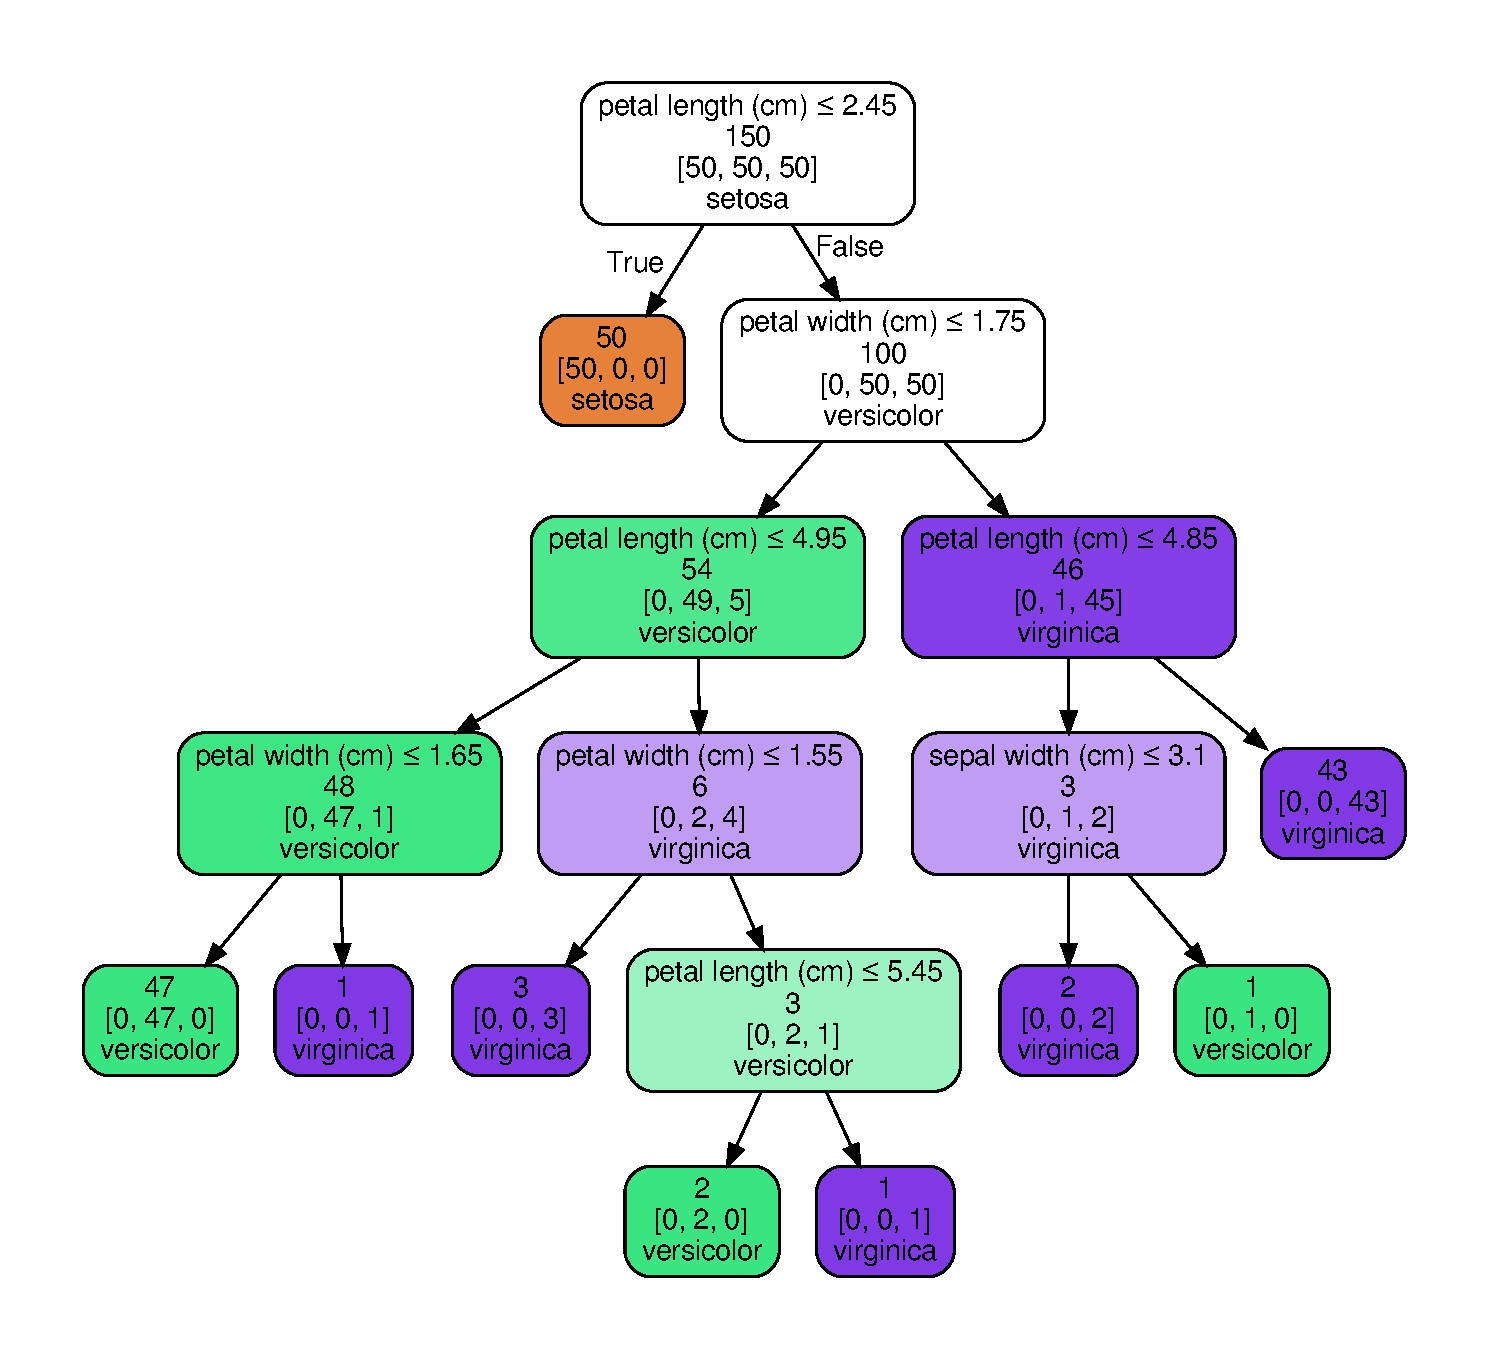
\includegraphics[width=0.75\textwidth, center, trim=0cm 0cm 0 0cm]{images/DT_6_simple.pdf}
	\end{figure}
\end{frame}

\begin{frame}{Decision Tree}
Decision Tree Decision Boundary
	\begin{figure}	
		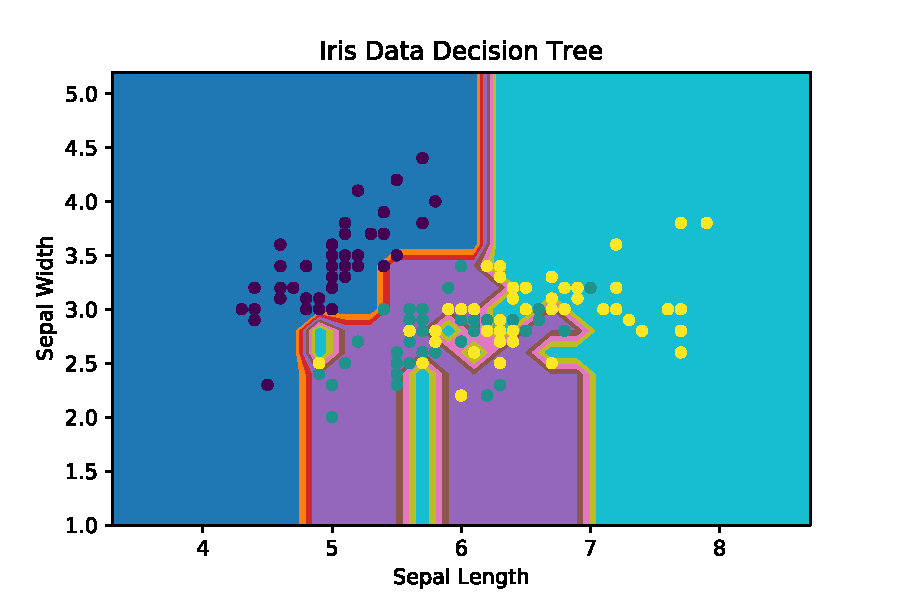
\includegraphics[width=0.9\textwidth, center, trim=0cm 0cm 0 0cm]{images/Iris_Data_DT.pdf}
	\end{figure}
\end{frame}

\begin{frame}{Decision Tree}
A method to fit data that generates reasonable decision boundaries
	\begin{itemize}
		\item Relatively fast and easy to fit
		\item Intuitive to use
		\item Often over fits data
			\begin{itemize}		
				\item Over fitting may be controlled with pruning
				\item Pruning may reduce accuracy
			\end{itemize}
		\item Large trees are difficult to interpret
	\end{itemize}
\end{frame}

\begin{frame}{Building a Forest of Decision Trees}
Make splits in the data in such a way that it separates the classes or that minimizes the distance between the predictions in a region.
		\begin{figure}	
			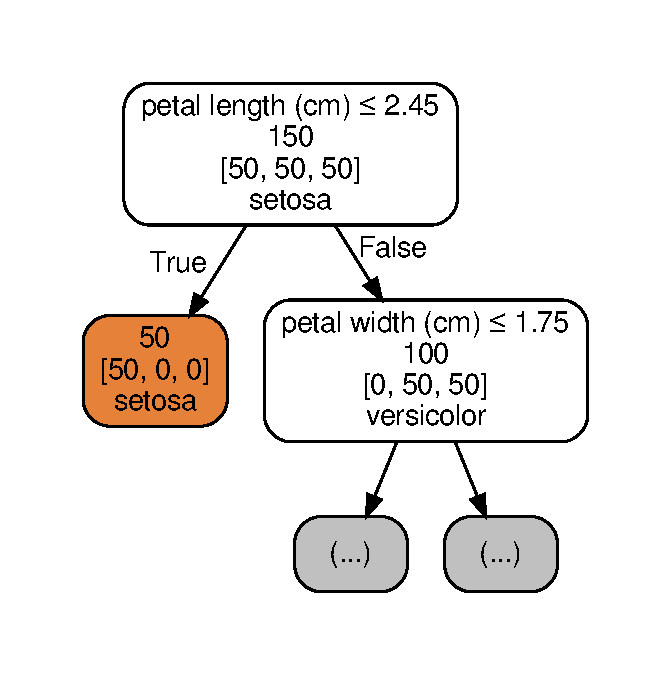
\includegraphics[width=0.55\textwidth, center, trim=0cm 0cm 0 0cm]{images/DT_2_simple.pdf}
	\end{figure}
\end{frame}

\begin{frame}{Random Forest}
\emph{Combine decision trees into an ensemble}
	\begin{columns}
	\begin{column}{0.5\textwidth}
	\begin{itemize}
		\item Work by randomly splitting predictors and data (bagging)
		\item Make a large number of trees and average their predictions
		\item Can be optimized with relatively few parameters
		\item Resulting models can be very large making inference slow
		\item Models do not fit sparse data well
		\item Results are difficult to interpret
	\end{itemize}
	\end{column}
	\begin{column}{0.5\textwidth}
		\begin{figure}
			\caption{Decision Tree Example}
			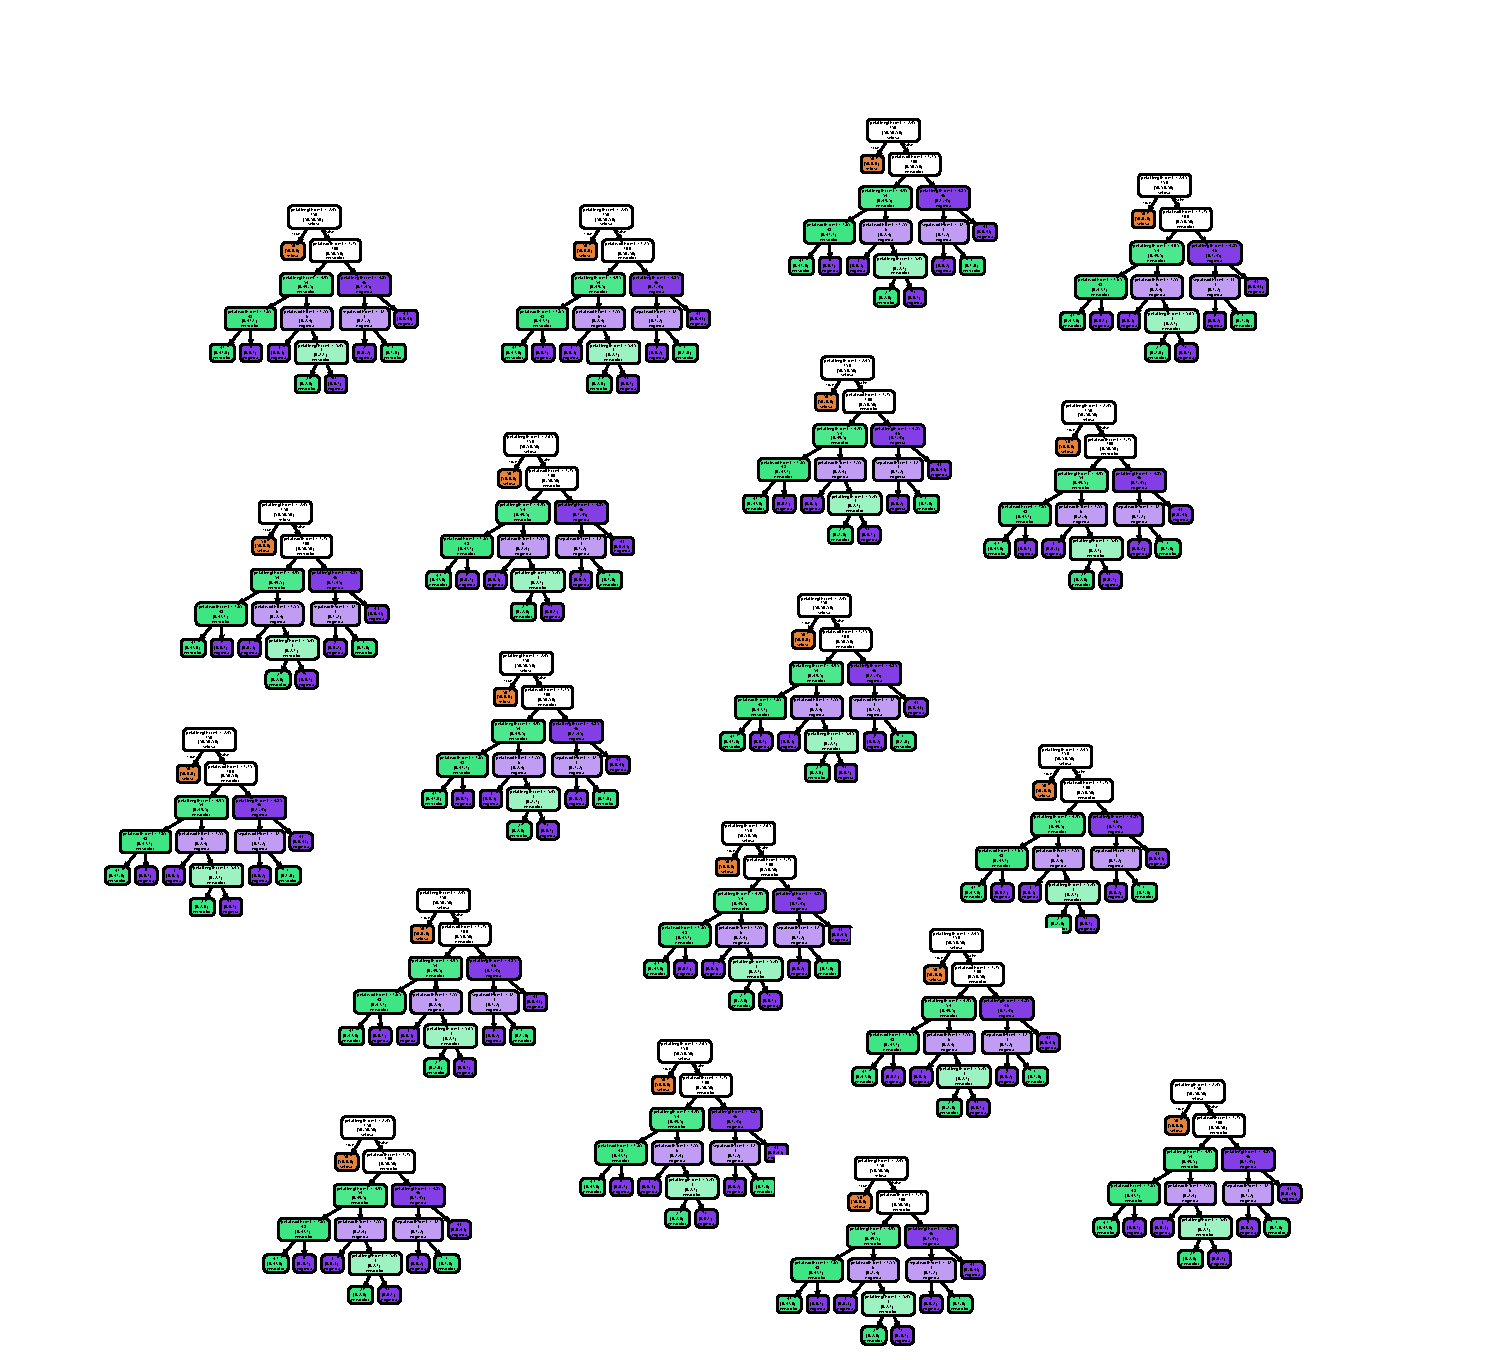
\includegraphics[width=1.0\textwidth, center, trim=1cm 0cm 0 0cm]{images/Random_forest.pdf}
	\end{figure}
	\end{column}
	\end{columns}
\end{frame}

\begin{frame}{Random Forest}
Random Forest Decision Boundary
		\begin{figure}	
			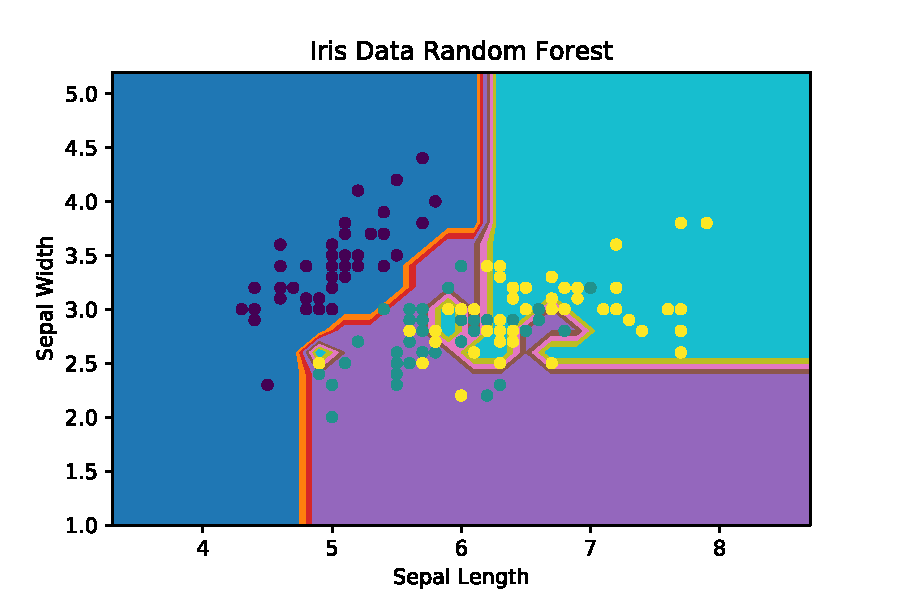
\includegraphics[width=1.0\textwidth, center, trim=0cm 0cm 0 0cm]{images/Iris_Data_RF.pdf}
	\end{figure}
\end{frame}

\begin{frame}{Boosted Trees}
\emph{Combine short decision trees fitting to the error of the previous tree}
	\begin{itemize}
		\item Make an ensemble of weak learners (small decision trees)
		\item Fit to decision trees to reduce the error of the previous tree
		\item Models generally have very high accuracy
		\item Over fitting is common
		\item Large number of difficult to optimize parameters
	\end{itemize}
\end{frame}

\begin{frame}{Boosted Trees}
GBM Decision Boundary
		\begin{figure}	
			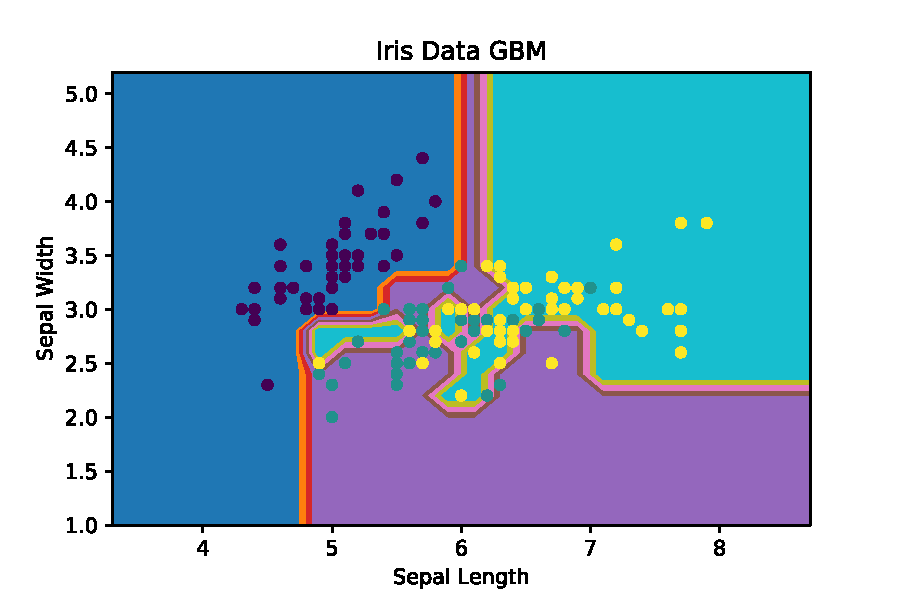
\includegraphics[width=1.0\textwidth, center, trim=0cm 0cm 0 0cm]{images/Iris_Data_GBM.pdf}
	\end{figure}
\end{frame}

\subsection{Neural Networks}
\begin{frame}{Neural Networks}
\emph{A class of models using collections of linear algebra operations to make predictions, classify data, so called deep learning and perform complex tasks}
	\begin{itemize}
		\item Wide-range of applications from classification to self-driving cars
		\item Automatic variable selection and engineering
		\item Require extensive fitting 
		\item Computationally intensive
		\item \alert{Many} architectures for different applications
		\item Applications include computer vision, natural language processing, predictions, task learning and speech recognition
		\item Fundamentally simple operations that when combined solve complex problems
	\end{itemize}
\end{frame}

\begin{frame}{Simplest Neural Network}
		\begin{figure}	
			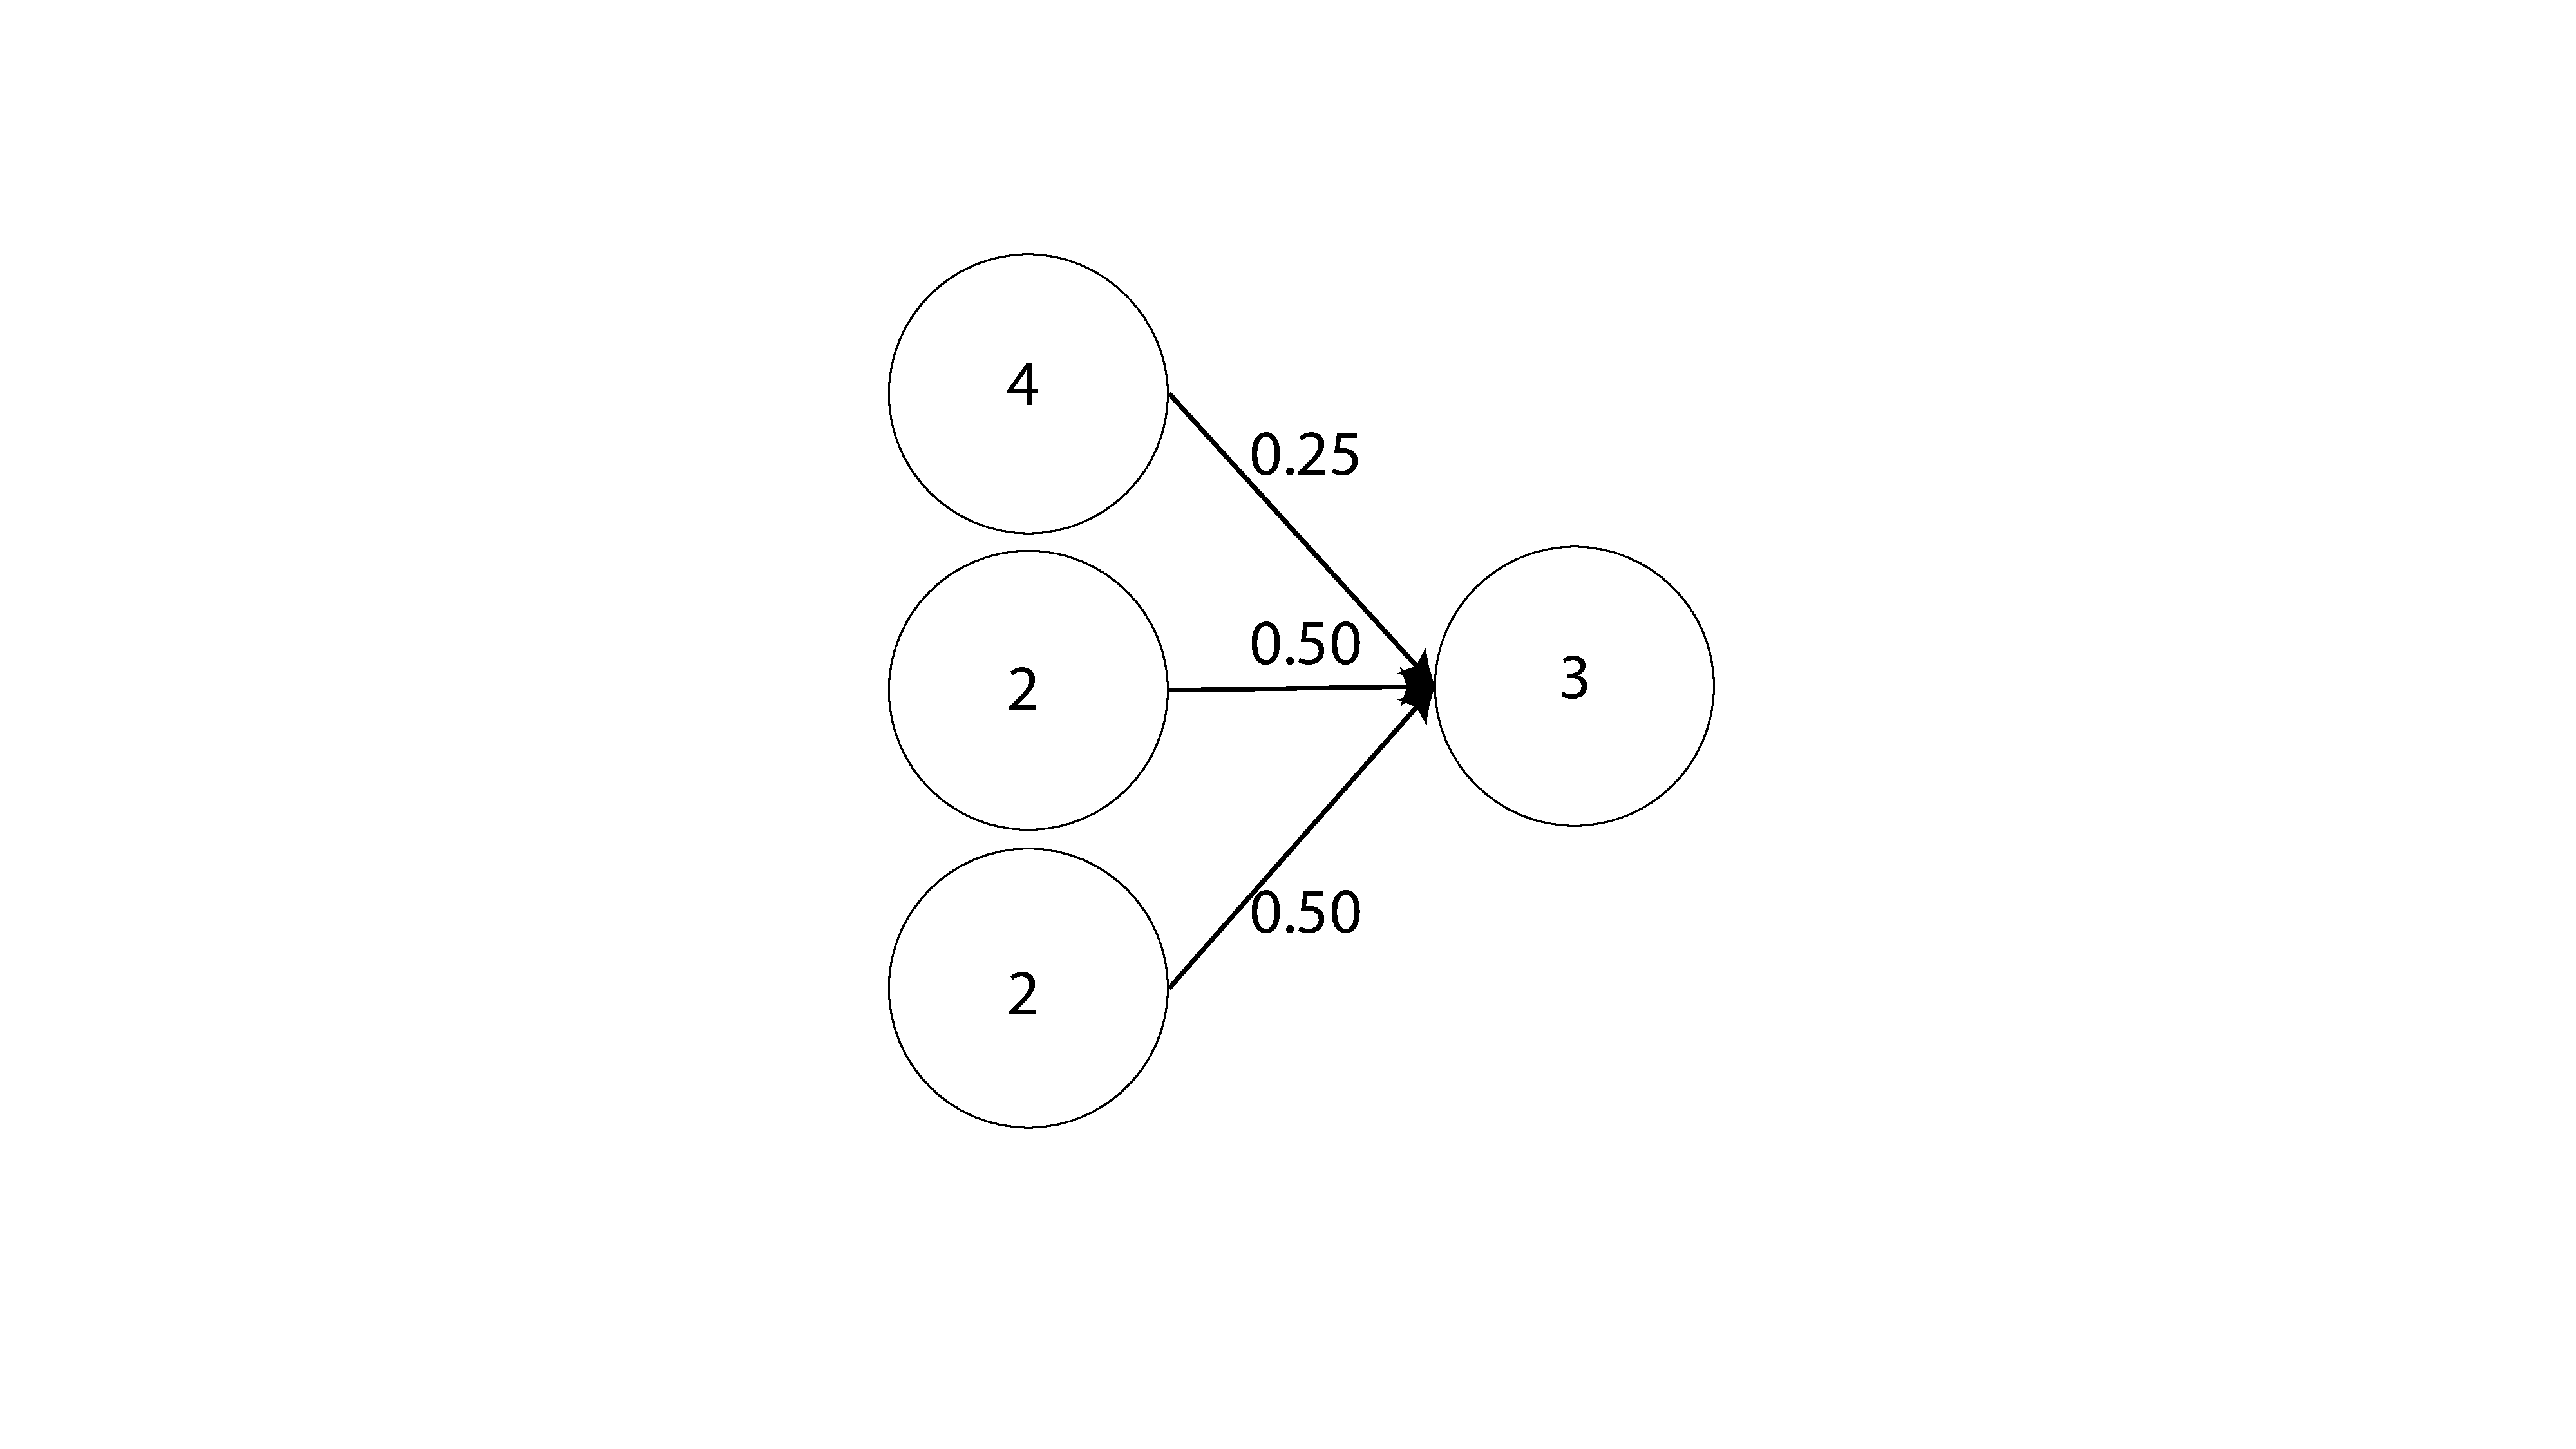
\includegraphics[width=1.5\textwidth, center, trim=0cm 0cm 0 0cm]{images/No_hidden_NN.pdf}
	\end{figure}
\end{frame}

\begin{frame}{Simplest Neural Network}
		\begin{figure}	
			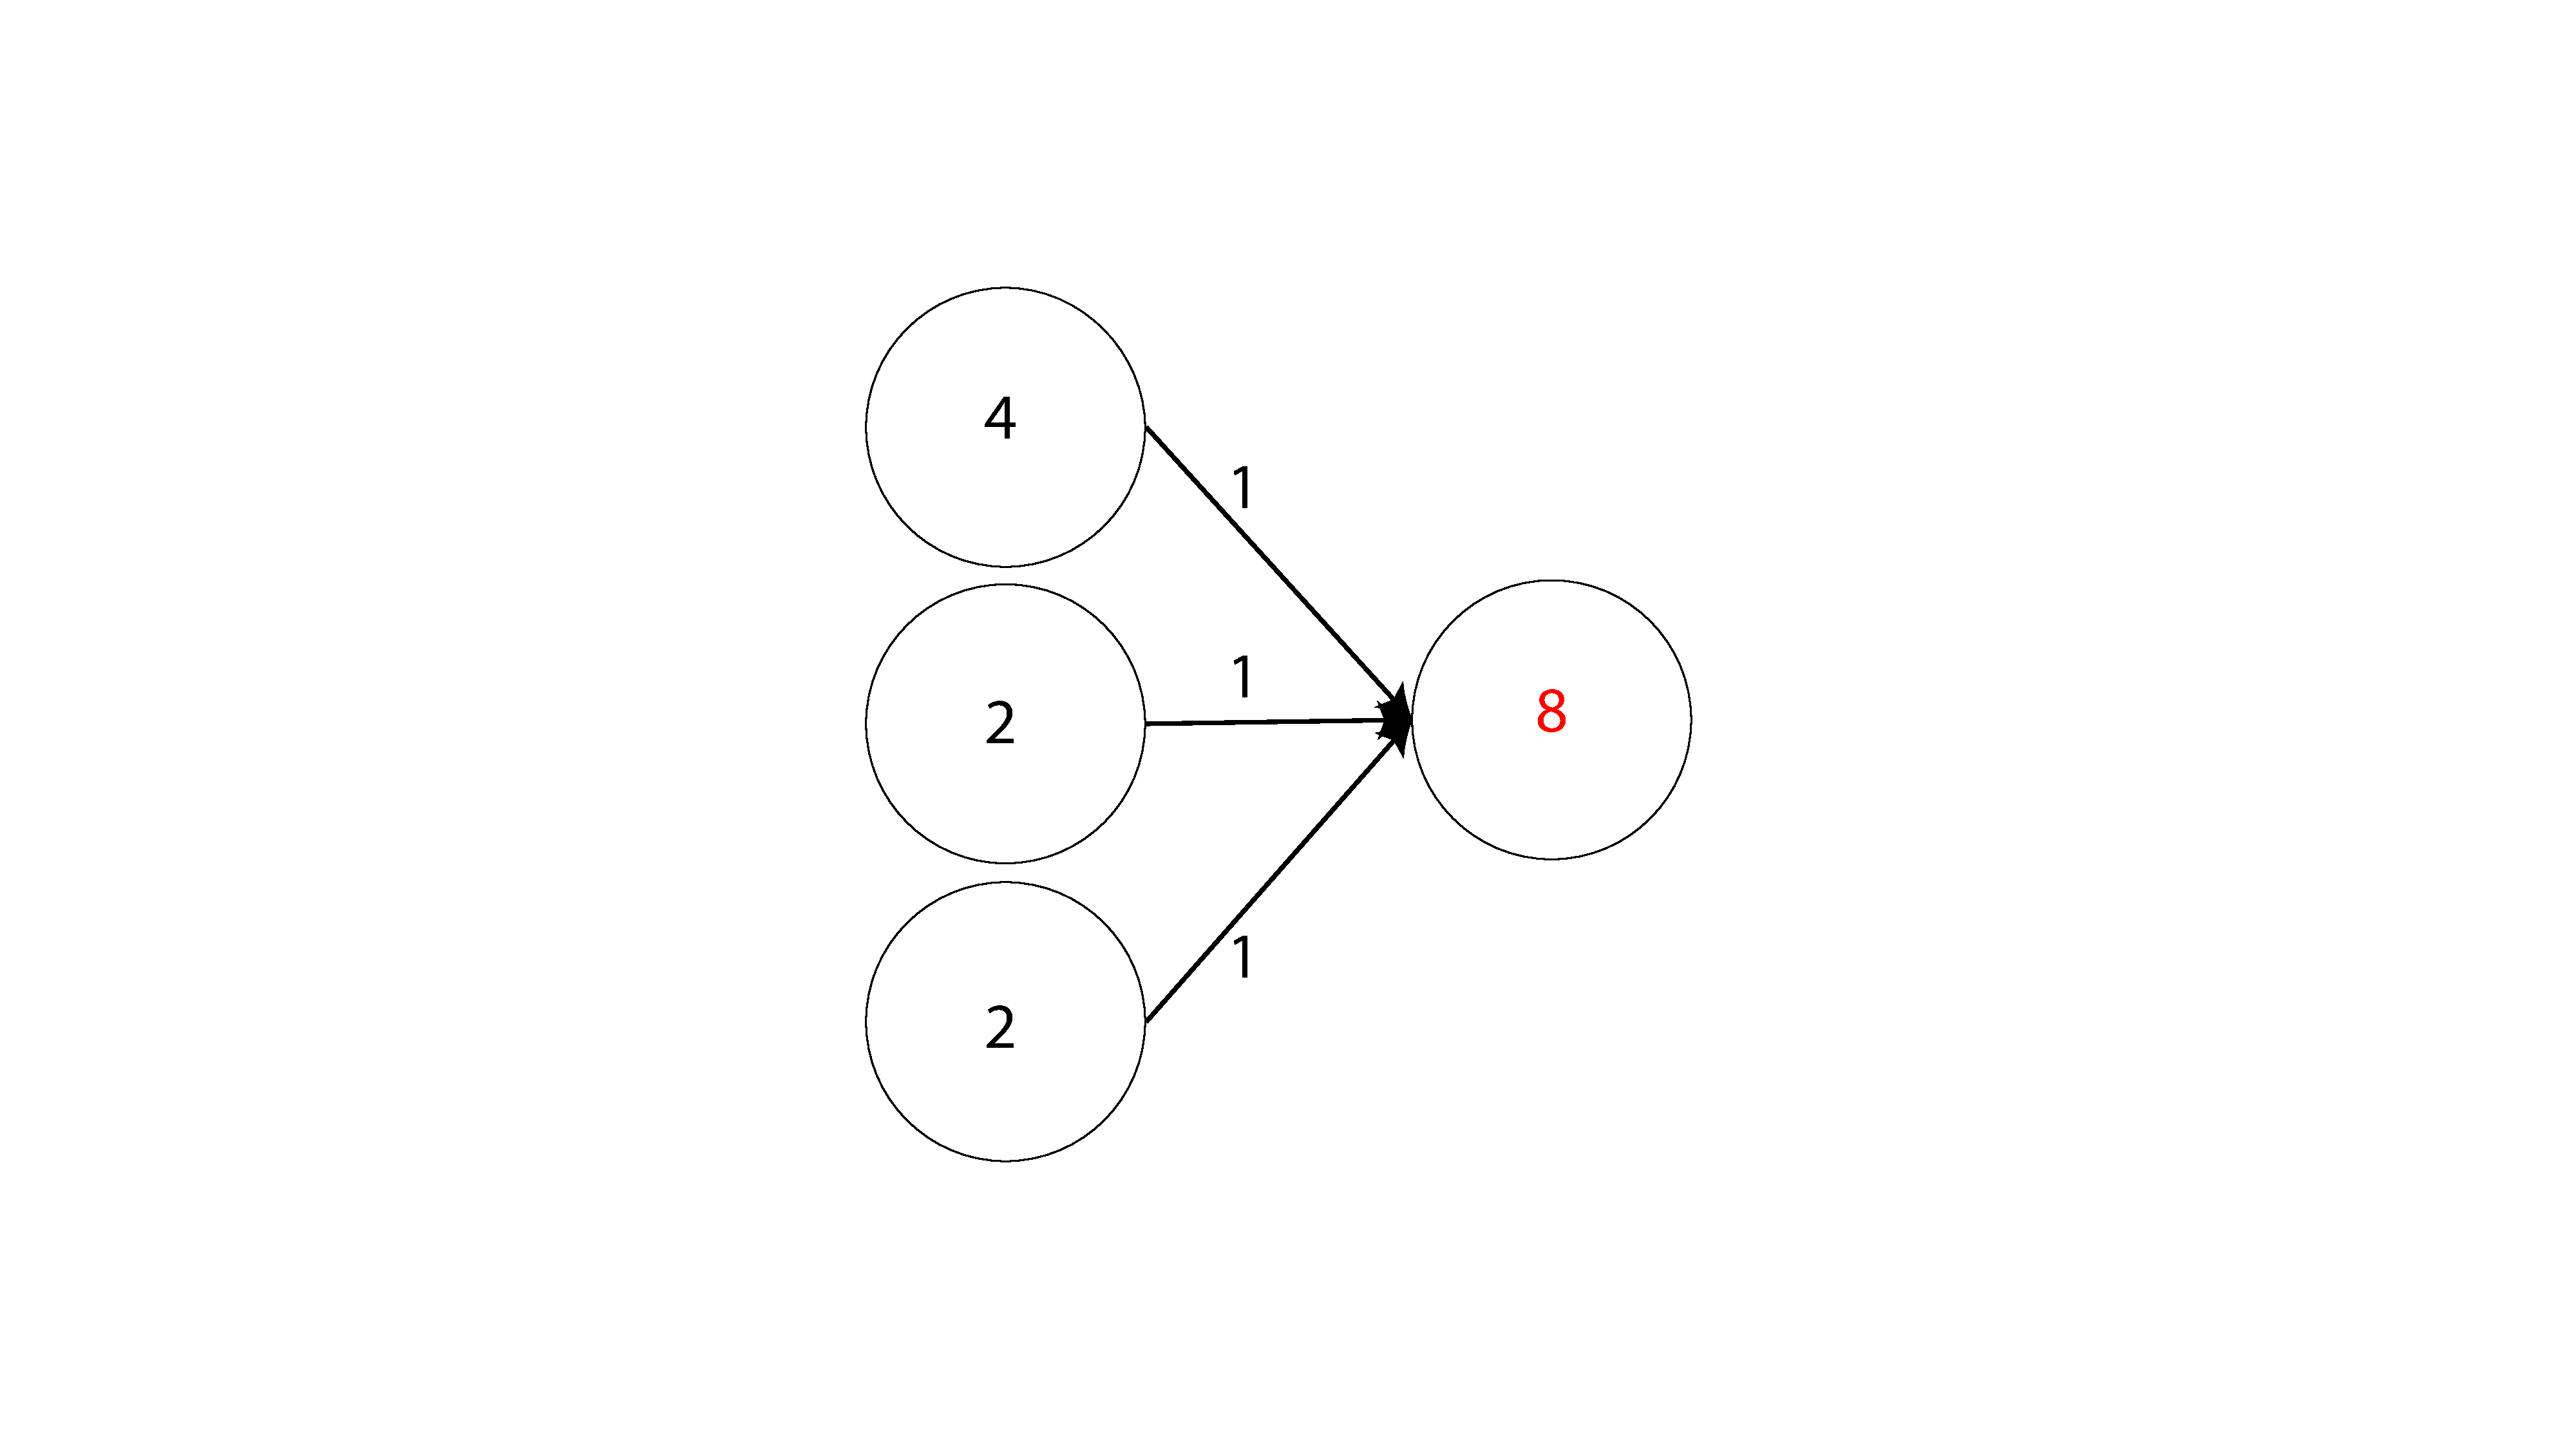
\includegraphics[width=1.5\textwidth, center, trim=0cm 0cm 0 0cm]{images/No_hidden_8W_NN.pdf}
	\end{figure}
\end{frame}

\begin{frame}{Simplest Neural Network}
		\begin{figure}	
			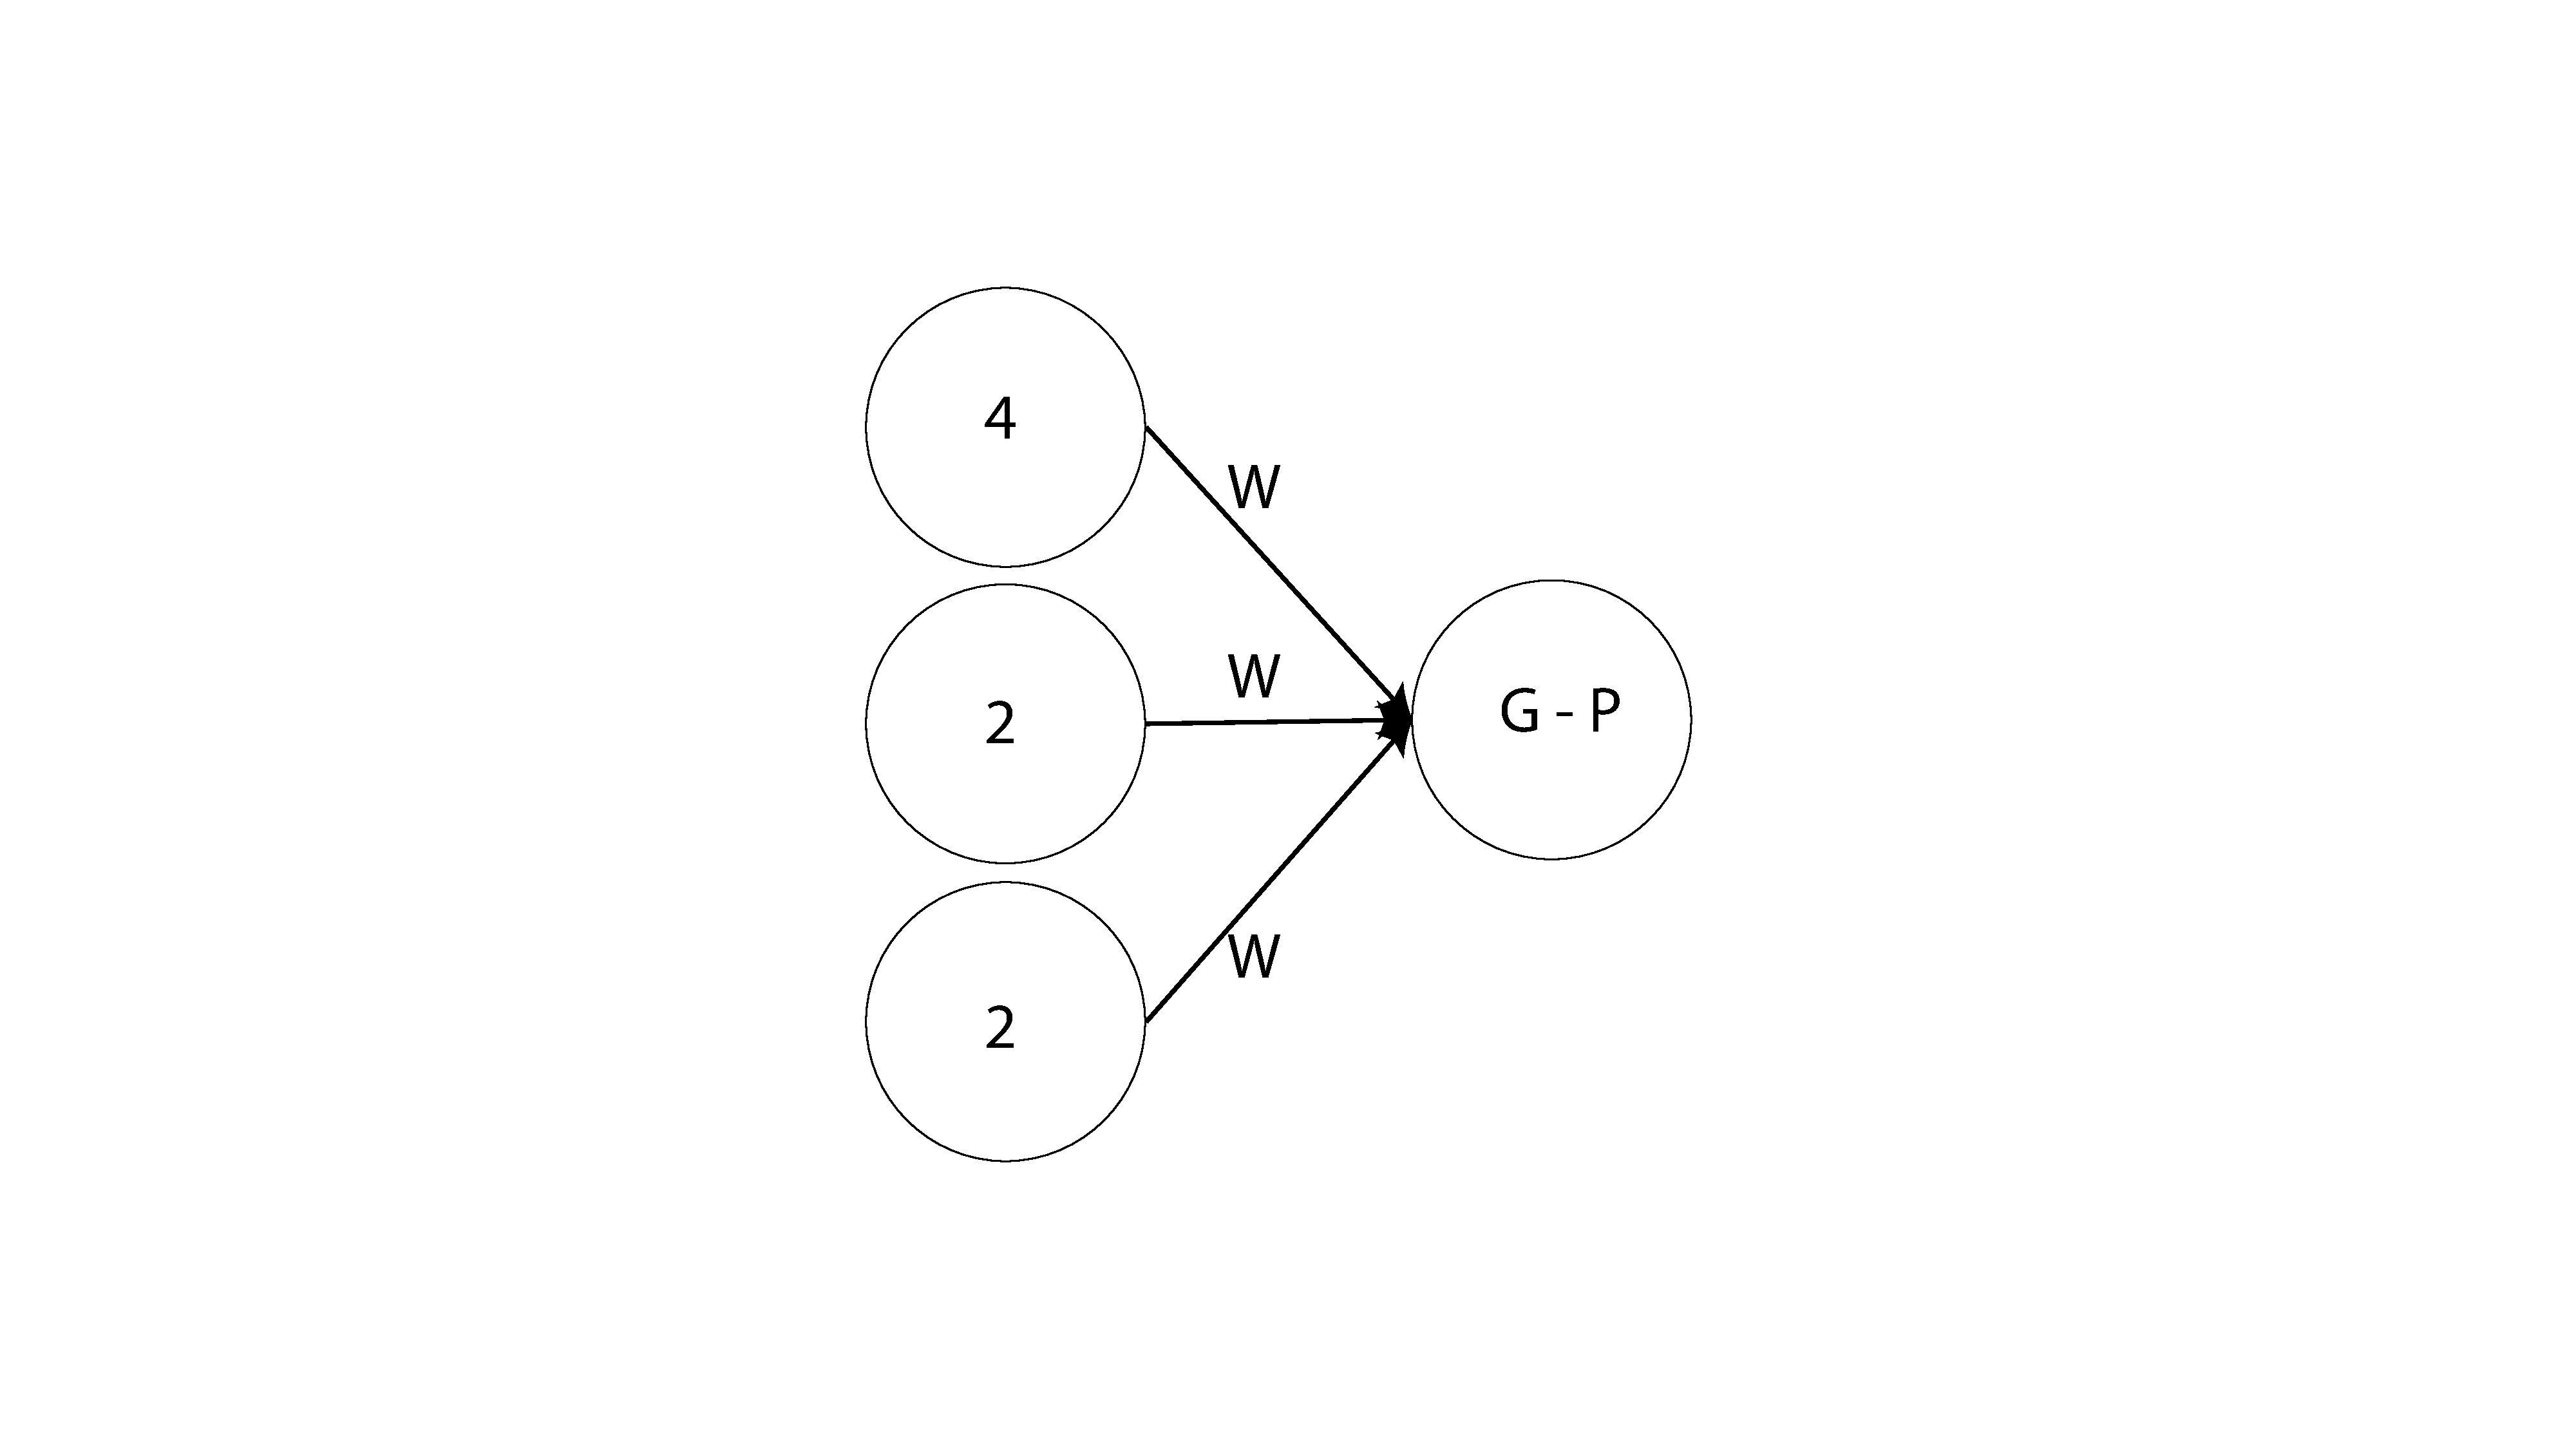
\includegraphics[width=1.5\textwidth, center, trim=0cm 0cm 0 0cm]{images/No_hidden_gen_NN.pdf}
	\end{figure}
\end{frame}

\begin{frame}{Simplest Neural Network}
		\begin{figure}	
			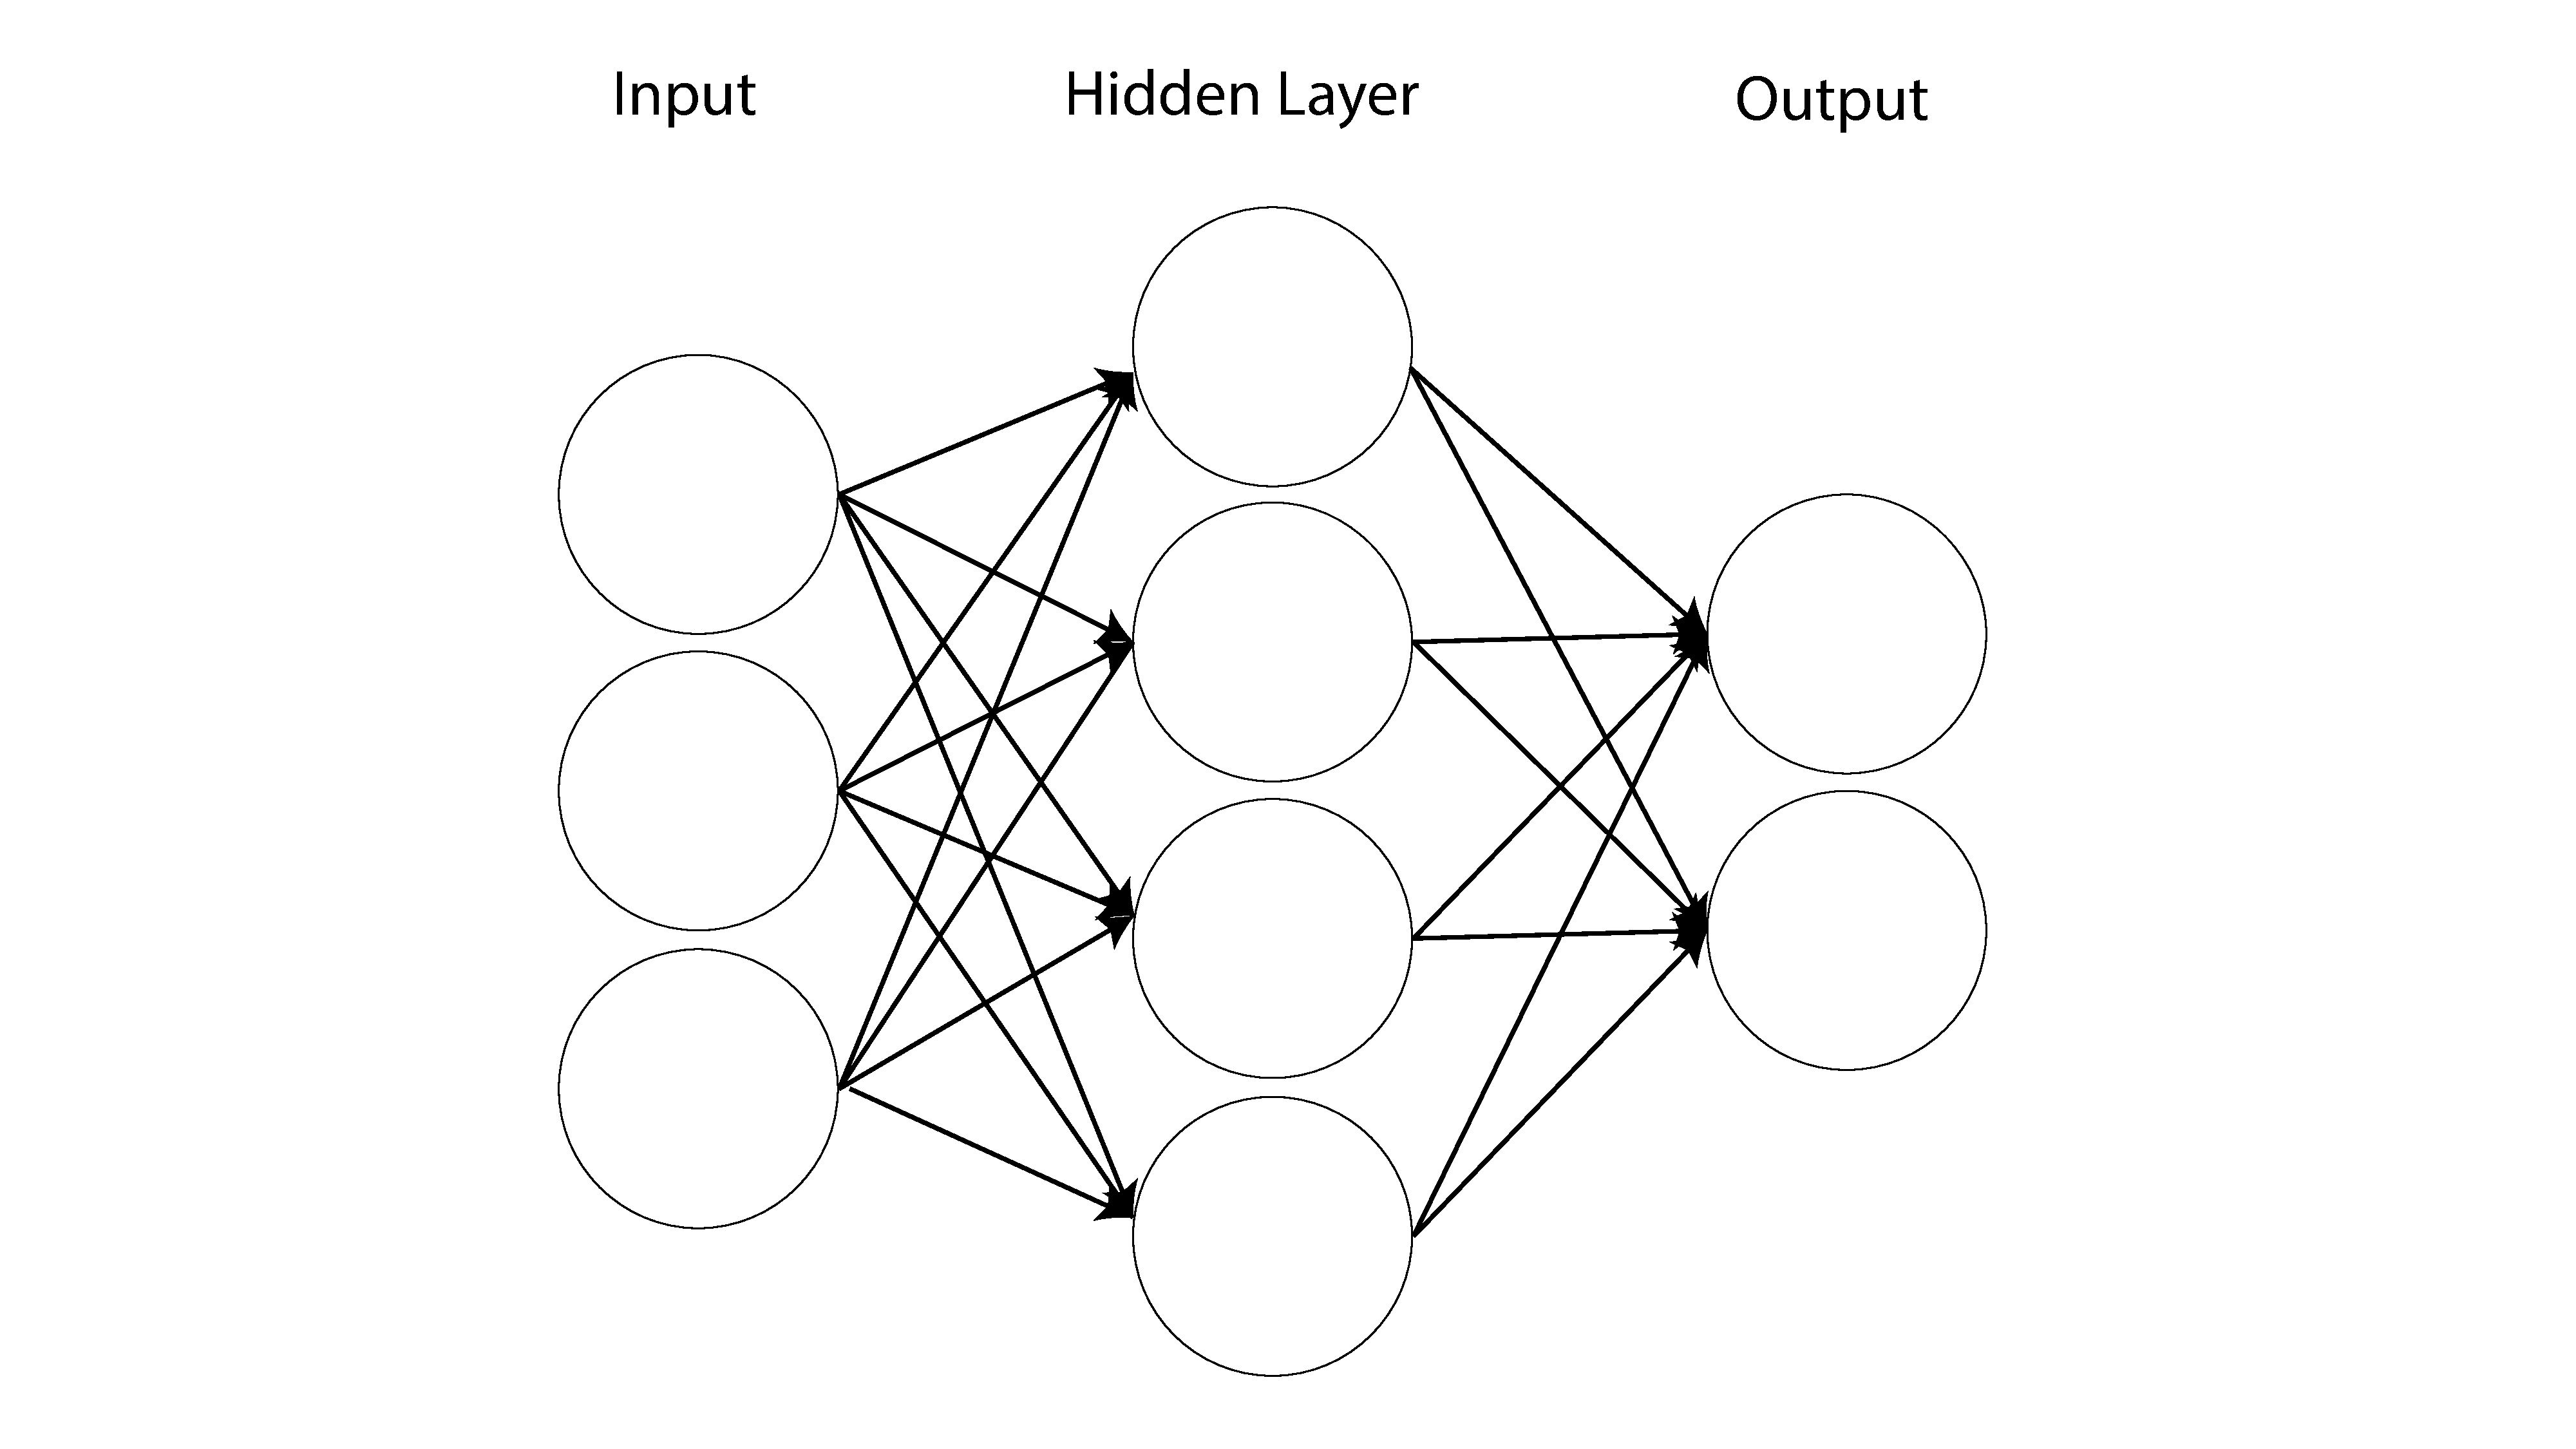
\includegraphics[width=1.0\textwidth, center, trim=0cm 0cm 0 0cm]{images/Dense_NN.pdf}
	\end{figure}
\end{frame}

\begin{frame}{Neural Network}
Neural Network Decision Boundary
		\begin{figure}
			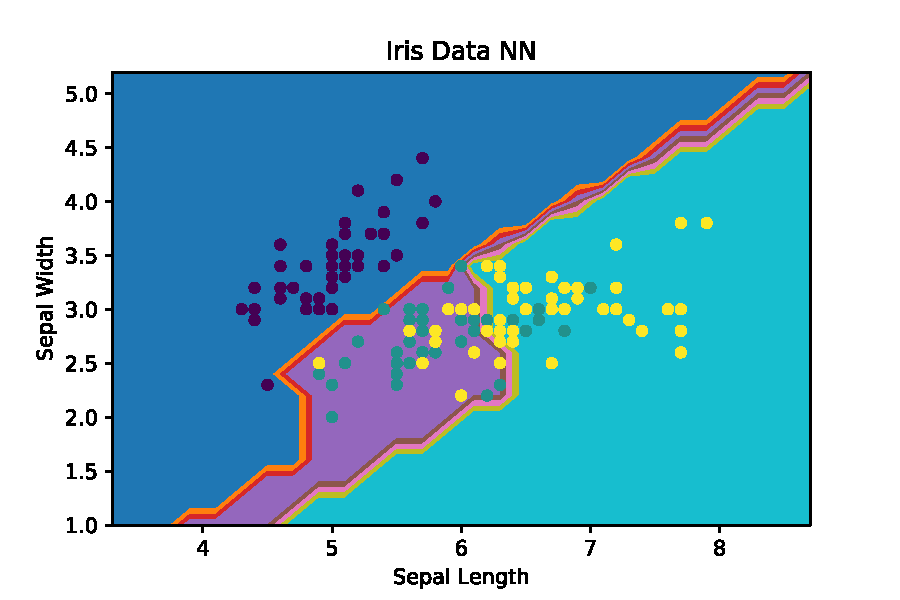
\includegraphics[width=0.9\textwidth, center, trim=0cm 0cm 0 0cm]{images/Iris_Data_NN.pdf}
	\end{figure}
\end{frame}

\subsection{Other}
\begin{frame}{Other Supervised Learning Methods}
\emph{Many other methods available}
	\begin{itemize}
		\item Regularized regression method to control overfitting and reduce variance
		\item Naive Bayes
		\item Gaussian Process
		\item Linear Discriminant Analysis
		\item k-Nearest Neighbors
	\end{itemize}
\end{frame}

\section{Unsupervised Learning}

\begin{frame}{Inferring the structure of unlabeled data}
\emph{Support Vector Machines and Decision Trees}
	\begin{itemize}
		\item Dimensionality Reduction
		\begin{itemize}
			\item Principle Component Analysis
			\item Non-negative Matrix Factorization
			\item Latent Dirichlet Allocation
		\end{itemize}
		\item Clustering
		\begin{itemize}
			\item K-means
			\item Gaussian Mixture Models
			\item Manifold Learning
		\end{itemize}
	\end{itemize}
\end{frame}

\subsection{Clustering}

\begin{frame}{PCA Dimensionality Reduction}
\emph{Find the best low dimensional representation of the data}
		\begin{figure}
			\caption{Iris Data with Three Components}
			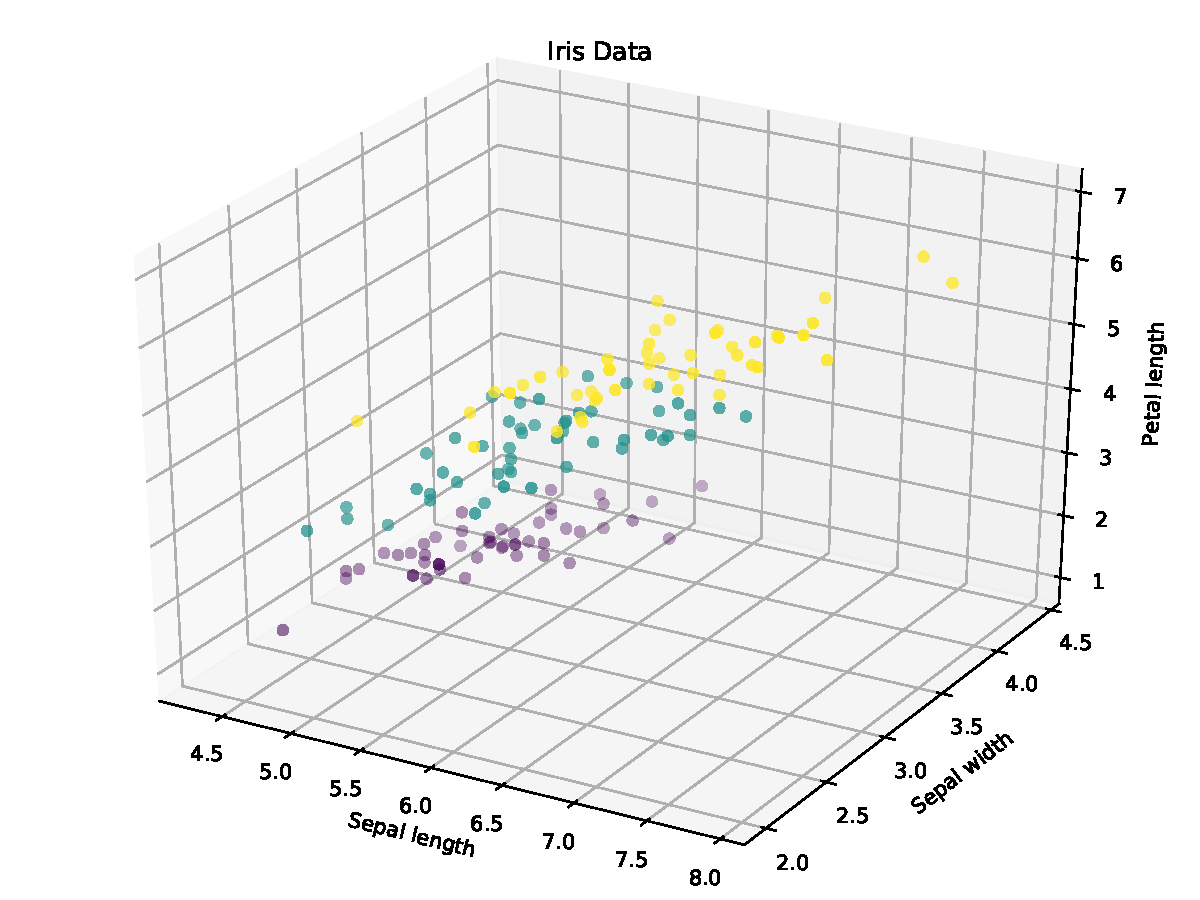
\includegraphics[width=0.75\textwidth, center, trim=0cm 0cm 0 0cm]{images/Iris_Data_3comp.pdf}
	\end{figure}
\end{frame}

\begin{frame}{PCA}
First two PCA eigenvectors
		\begin{figure}	
			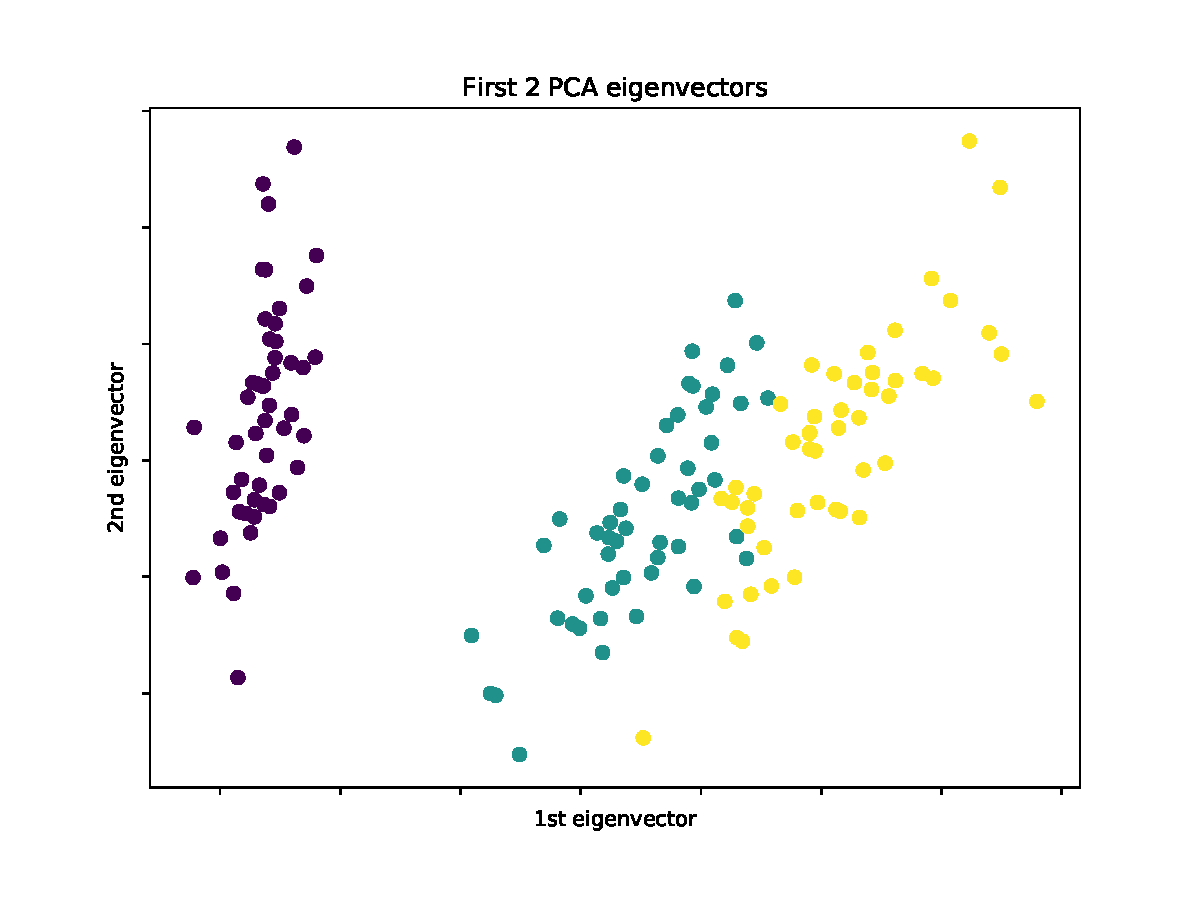
\includegraphics[width=0.75\textwidth, center, trim=0cm 0cm 0 0cm]{images/Iris_PCA.pdf}
	\end{figure}
\end{frame}

\begin{frame}{K-means}
\emph{Find K groupings based on variable similarity.}
		\begin{figure}
			\caption{Iris Data with 3 cluster}
			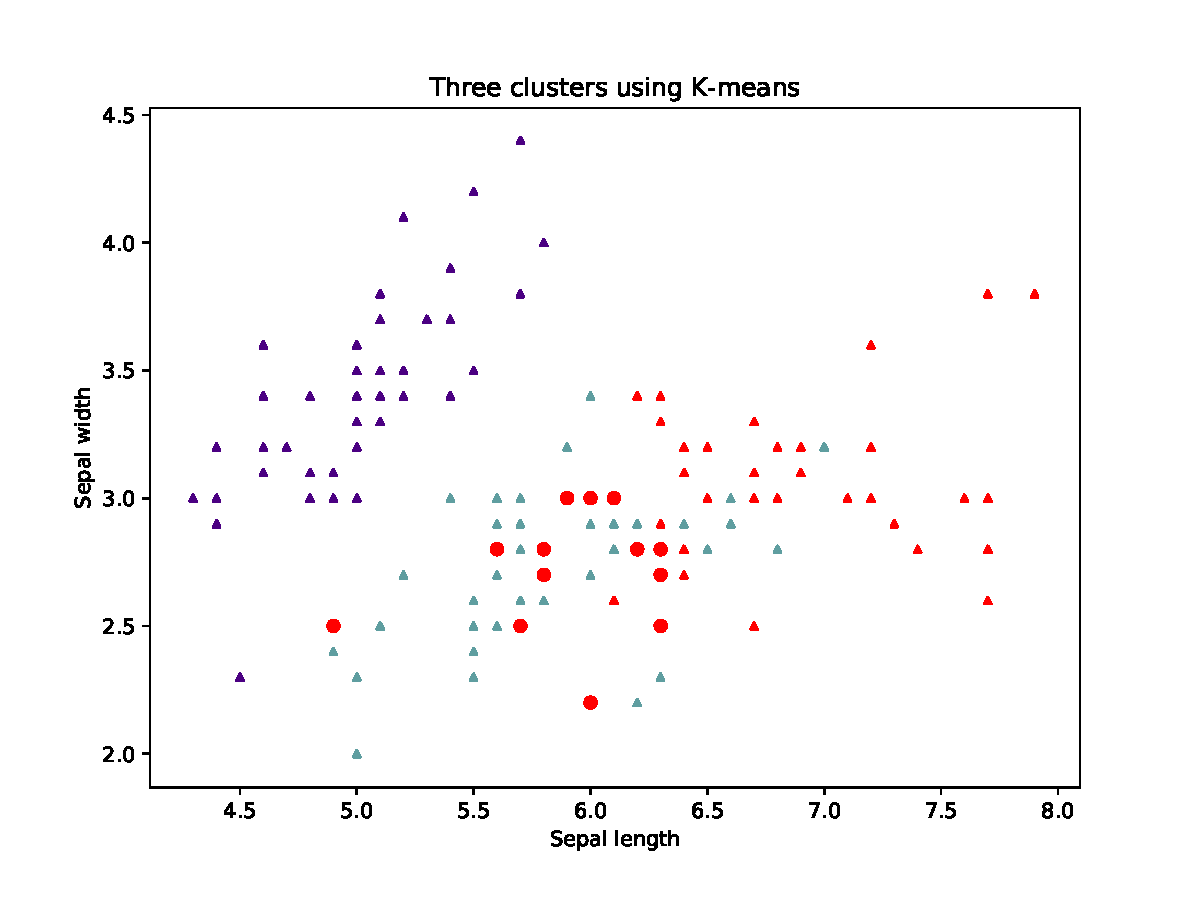
\includegraphics[width=0.75\textwidth, center, trim=0cm 0cm 0 0cm]{images/Iris_3means.pdf}
	\end{figure}
\end{frame}

\section{Reinforcement Learning}

\begin{frame}{New problem types}
\emph{What if we know the desired outcome but the data needed to model every possible situation is vast or there the decision is dependent on many changing factors?}
	\begin{itemize}
		\item Reinforcement learning is a method to learn a policy to arrive at an outcome rather than learning a labeled value
		\item Successes include self-driving cars, beating the best in the world at the game of Go and playing most Atari games at superhuman levels 
		\item Must define the actions, the rewards and the states
		\item Very data intense
	\end{itemize}
\end{frame}

\begin{frame}{Reinforcement Learning Concept}
\emph{What if we know the desired outcome but the data needed to model every possible situation is vast or there the decision is dependent on many changing factors?}
		\begin{figure}
			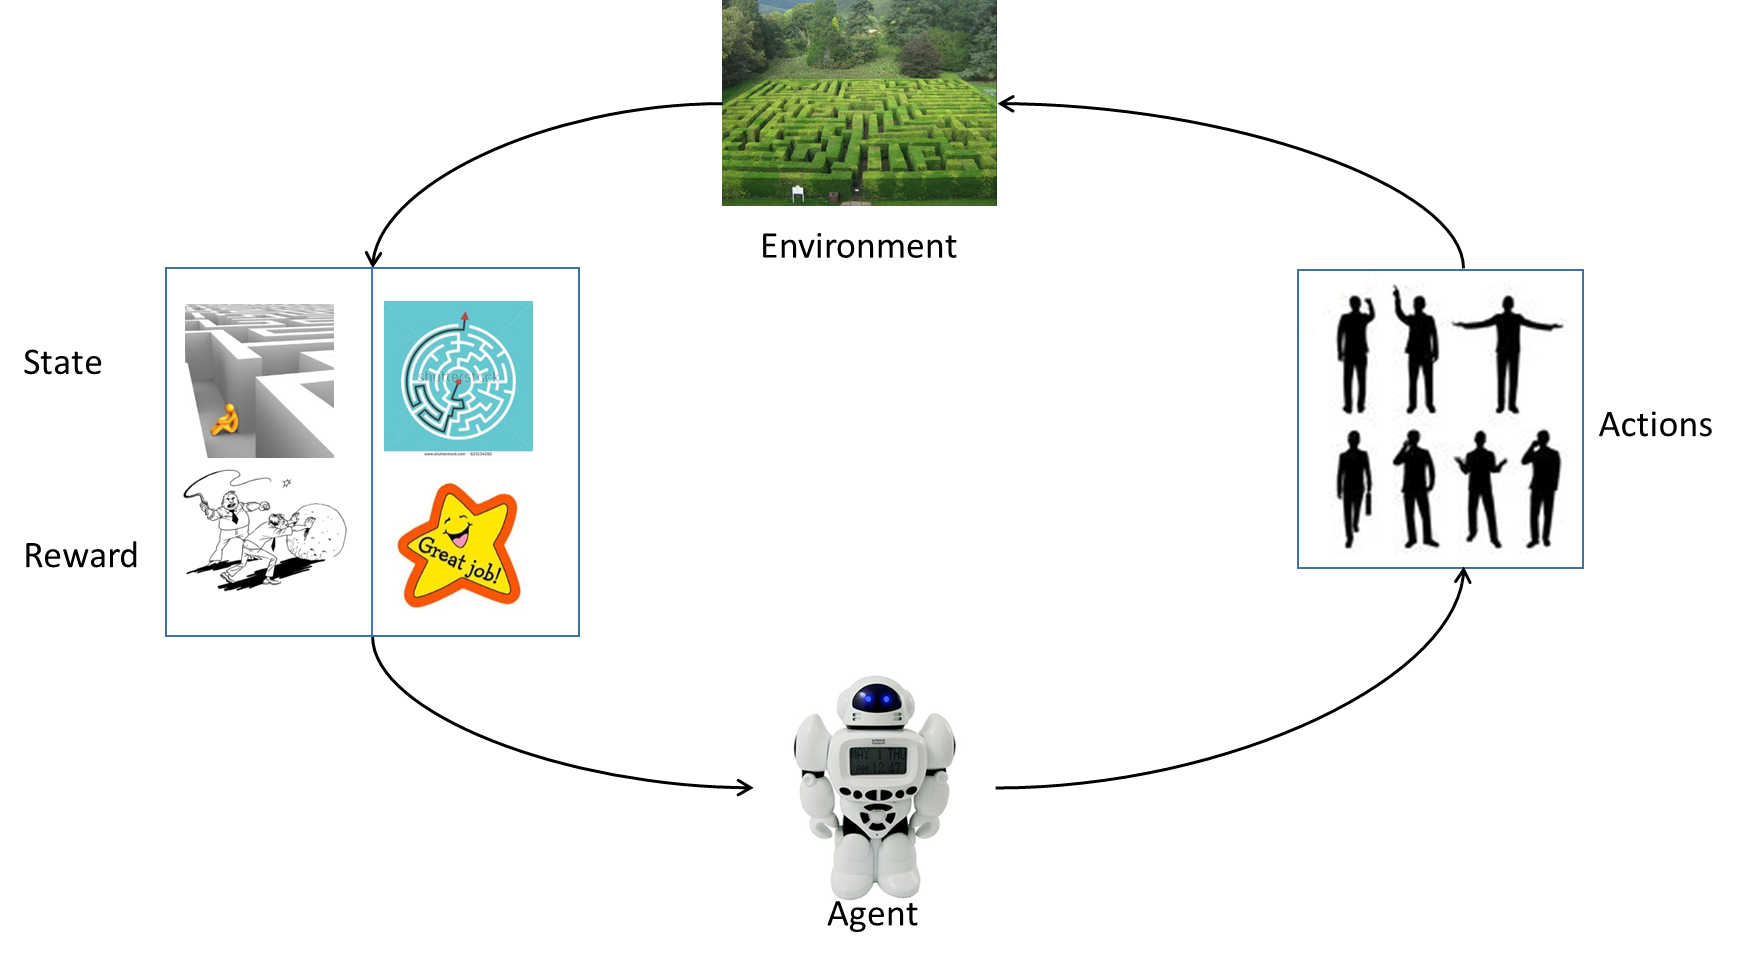
\includegraphics[width=1.00\textwidth, center, trim=0cm 0cm 0 0cm]{images/RL_concept.png}
	\end{figure}
\end{frame}

\begin{frame}{Reinforcement Learning Example}
\emph{Self-Driving Race Car}
		\begin{figure}
			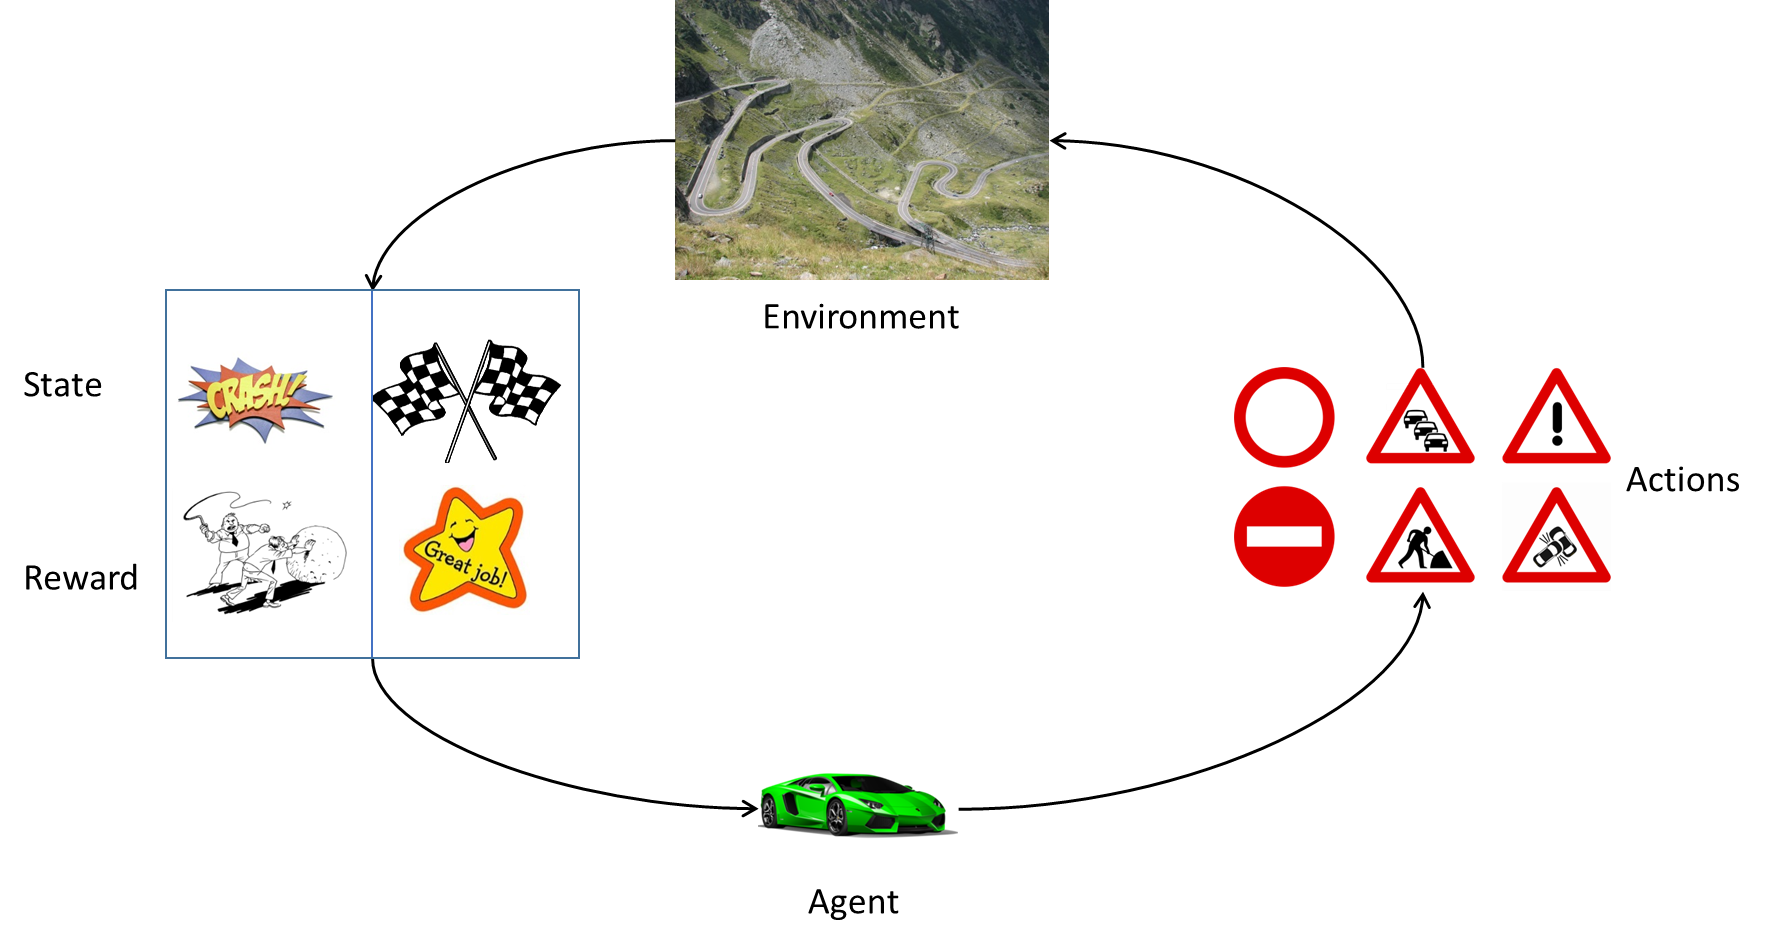
\includegraphics[width=1.00\textwidth, center, trim=0cm 0cm 0 0cm]{images/RL_example.png}
	\end{figure}
\end{frame}

\section{Special Topics}

\subsection{Natural Language Processing}

\begin{frame}{Teaching a computer to read}
\emph{Computers can't read! Wait can they?} \\~\\
London is the capital and most populous city.
	\begin{figure}
		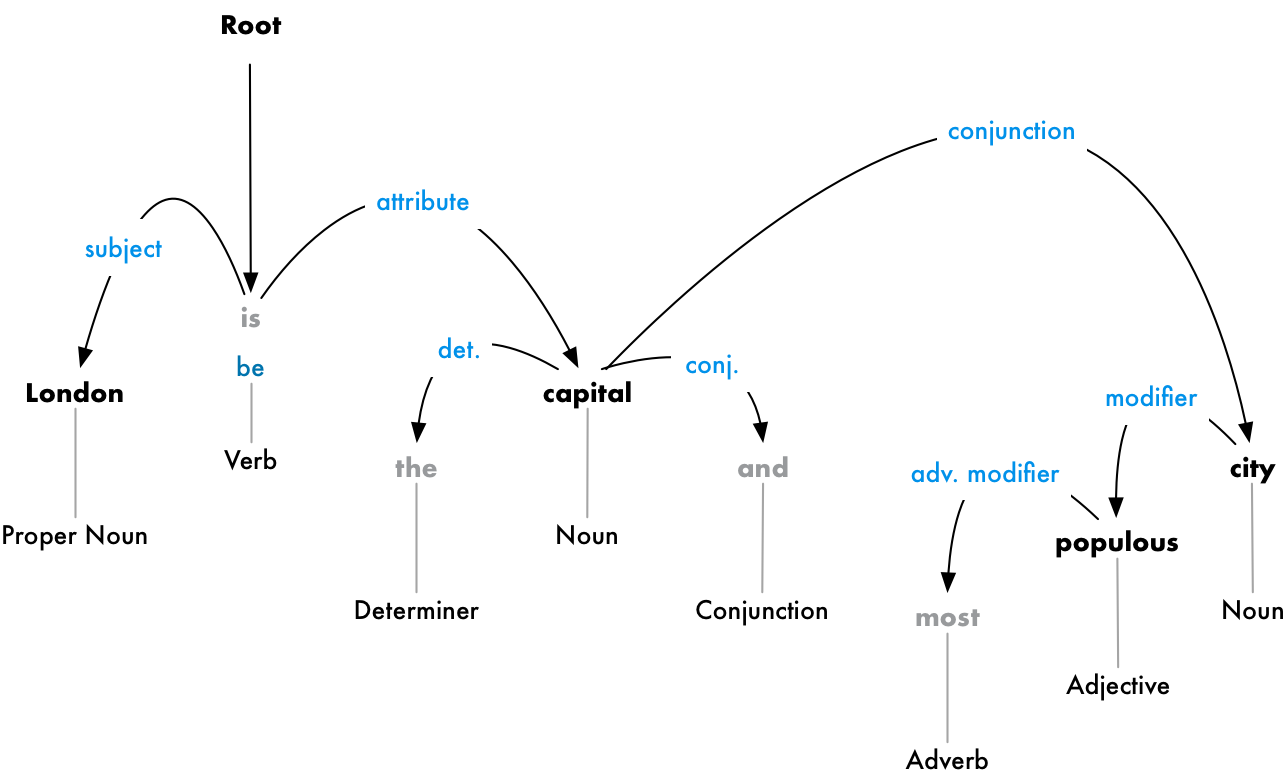
\includegraphics[width=0.95\textwidth, center, trim=0cm 0cm 0 0cm]{images/NLP_tree.png}
	\end{figure}

\end{frame}

\subsection{Computer Vision}

\begin{frame}{How do computers see?}
\emph{What about images? What would a machine learning algorithm use to add the labels below?}	
	\begin{figure}
		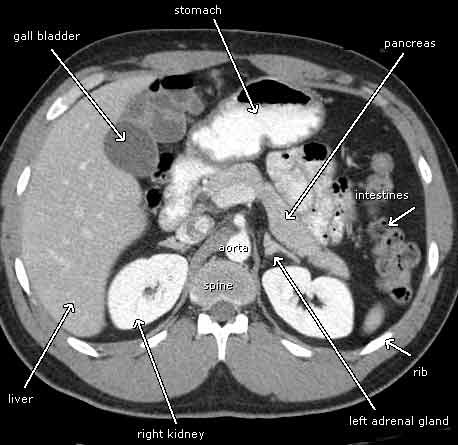
\includegraphics[width=0.65\textwidth, center, trim=0cm 0cm 0 0cm]{images/CT_scan.jpeg}
	\end{figure}

\end{frame}

\end{document}